% REMEMBER: You must not plagiarise anything in your report. Be extremely careful.
\documentclass{l4proj}

    
%
% put any additional packages here
%
\begin{document}

%==============================================================================
%% METADATA
\title{Visual Field Testing in Virtual Reality with Eye Tracking and Visual Feedback}
\author{Alfie J. Macintosh}
\date{March 29th, 2024}

\maketitle

%==============================================================================
%% ABSTRACT
\begin{abstract}
    Every abstract follows a similar pattern. Motivate; set aims; describe work; explain results.
    \vskip 0.5em
    ``XYZ is bad. This project investigated ABC to determine if it was better. 
    ABC used XXX and YYY to implement ZZZ. This is particularly interesting as XXX and YYY have
    never been used together. It was found that  
    ABC was 20\% better than XYZ, though it caused rabies in half of subjects.''
\end{abstract}

%==============================================================================

% EDUCATION REUSE CONSENT FORM
% If you consent to your project being shown to future students for educational purposes
% then insert your name and the date below to  sign the education use form that appears in the front of the document. 
% You must explicitly give consent if you wish to do so.
% If you sign, your project may be included in the Hall of Fame if it scores particularly highly.
%
% Please note that you are under no obligation to sign 
% this declaration, but doing so would help future students.
%
\def\consentname {Alfie J. Macintosh} % your full name
\def\consentdate {7 February 2024} % the date you agree
%
\educationalconsent


%==============================================================================
\tableofcontents

%==============================================================================
%% Notes on formatting
%==============================================================================
% The first page, abstract and table of contents are numbered using Roman numerals and are not
% included in the page count. 
%
% From now on pages are numbered
% using Arabic numerals. Therefore, immediately after the first call to \chapter we need the call
% \pagenumbering{arabic} and this should be called once only in the document. 
%
% Do not alter the bibliography style.
%
% The first Chapter should then be on page 1. You are allowed 40 pages for a 40 credit project and 30 pages for a 
% 20 credit report. This includes everything numbered in Arabic numerals (excluding front matter) up
% to but excluding the appendices and bibliography.
%
% You must not alter text size (it is currently 10pt) or alter margins or spacing.
%
%
%==================================================================================================================================
%
% IMPORTANT
% The chapter headings here are **suggestions**. You don't have to follow this model if
% it doesn't fit your project. Every project should have an introduction and conclusion,
% however. 
%
%==================================================================================================================================
\chapter{Introduction}
[FILL WHAT IS MY PROJECT] ALTHOUGH CONTEMPRY SYSTEMS HAVE DONE THIS, FUNDAMENTAL DRAWBACKS MREAN I HAVE TRIED TO IMPLEMENT THIS
% reset page numbering. Don't remove this!
\pagenumbering{arabic} 
\section{Motivation}
Visual field testing plays a crucial role in assessing the visual health of patients. It is often used as a diagnostic tool by neuro-ophthalmologists, specialists dealing with visual problems related to the nervous system. By measuring a patients visual field, clinicians can diagnose and track the progress of a wide range of conditions affecting vision, from glaucoma to neurological conditions. 

However, traditional visual field tests present a number of challenges in terms of accessibility and patient compliance. Traditional machinery to conduct a visual field test are often both expensive and limited in availability. Furthermore, human-error and non-compliance with testing procedures can compromise the accuracy and validity of tests. 

As a result of this, there is a need for an innovative solution that enhances user experience, accuracy and reliability. By leveraging the technology that is currently present in commercial virtual reality headsets, we aim to alleviate the problems currently faced in visual field testing. Virtual reality offers the potential to make visual field testing more accessible, cost-effective and engaging for users while improving the reliability and accuracy of results by utilising eye tracking technology and providing real-time visual feedback to the user.

Utilising virtual reality as a platform for performing visual field testing has seen some promise in clinical trials. \cite{Stapelfeldt2021VRGlaucoma} conducted a study comparing virtual reality-based visual field testing to traditional methods and found that their virtual reality system performed comparably to current visual field machines. Additionally, a study by \cite{Wroblewski2014TestingVisualField} found there was minimal systematic differences between their virtual reality system, VirtualEye, and traditional visual field testing machines.

\section{Aims}
Our primary aim is to develop and evaluate a visual field testing platform in virtual reality that incorporates real-time visual feedback functionality. Leveraging the eye-tracking technology in our headset, this system will provide immediate feedback to our users during the testing process to help inform them of their compliance to test procedure. By integrating this feature, we hypothesis that the validity of tests will increase, where as the validity of testing without this functionality will not perform as well when we compare these test conditions.

To evaluate the impact of visual feedback we will conduct a user evaluation and use the data from this evaluation to validate the performance of our system. These evaluations will focus on quantifying improvements in key test outcomes such as fixation loss, false positives and false negatives. Additionally it is important understand the usability of the system, and so we will consider factors such as comfort and overall user experience.

Furthermore it is important to understand how the system is perceived by users with neuro-ophthalmic conditions and users with other visual impairments. Hence, we will conduct an individual study on a user with right-side homonymous Hemianopia (see \ref{background:VFT_Hemianopia}).

By perusing these aims our we endeavor to see if these features enhance the reliability of visual field testing while ensuring the usability of our system.
\section{Content Outline}
This section provides an overview of this papers structure, summarising each chapters contents. Please see below for each chapters summary:
\begin{itemize}
    \item \textbf{Background}: This first chapter provides the context for the rest of the paper. It includes information on past attempts, as well as information on current testing protocol, so the user can understand the motivation for researching this particular topic.
    \item \textbf{Analysis/Requirements}: This chapter outlines the problem statement. Additionally, it breaks down our problem statement into attainable functional and non-functional requirements for our design and implementation chapters.
    \item \textbf{Design}: This chapter outlines the systems architecture, in abstracted terms. It includes information on this projects setup and provides guidance on how the program can be implemented.
    \item \textbf{Implementation}: In this chapter we outline how this project has actually been developed using our design. Furthermore, it highlights the hardware required to run this program as well as how supporting packages have enabled this implementation.
    \item \textbf{Evaluation}: This chapter provides the methodology of our user evaluation. It discusses the results we collated from our user evaluation survey and data collected during user testing. Furthermore, by using this data we can confirm or reject our hypothesis that visual feedback will improve validity of our testing.
    \item \textbf{Conclusion}: Finally, in this chapter we summarise our paper and its findings, while laying out possible future work.
\end{itemize}



%==================================================================================================================================
\chapter{Background}
\section{Visual Field Testing}
Visual Field Testing is a diagnostic tool used in ophthalmology and neurology to evaluate a persons field of vision. It can be used to assess both the central and peripheral vision, to identify Scotomas (blind spots), areas of diminished vision or areas of complete loss of vision \citep{AAO2021VisualField}. Results from visual field testing can be used to diagnose eye and brain conditions, including glaucoma, retinal detachment and strokes or tumors. The abnormalities in the results can further be used by healthcare professionals to guide treatment decisions and monitor disease progression. 

Methods of Visual field testing have evolved over the years. From one of the first peripheral visual field evaluations which described Hemianopia by Hippocrates \citep{Johnson2011Perimetry} in the 5th Century B.C., to the breakthrough work of Hans Goldmann who in 1946 created the Goldmann machine. He created a semispherical bowl that had uniform background illumination and would superimpose stimuli in the background. A stimulus would be manually moved from beyond the edge of the users visual field until they could see it, at which point it would showcase the users visual field outer perimeter. While a breakthrough at the time, today it has been overtaken by automated perimetry due to the inter-test variability challenge \citep{CarrollJohnsonVFTutorial2021}. Inter-test variability, in the context of visual field testing, refers to the variability in test results when the same users visual field is tested. This is caused by a number of factors, one such factor is that traditional machines were completely human operated and thus susceptible to human error.




\subsection{Automated Perimetry}
Automated Perimetry advanced previous methods of visual field testing introducing a repeatability and efficiency previously not possible. Developed n the early 1970s by Drs G. Lynn and G. Tate \citep{HKMJ2023}. This technology utilises computer-controlled equipment to present stimuli at points in the visual field to systematically map the patients visual capabilities, identifying areas of impairment or loss in vision.

The test involved patients sitting in front a concave dome while focusing on a central point. The computer would then present stimuli of varying intensities at random locations. The patient would indicate their perception of the stimuli by clicking a button which would be used by the system to map their visual field. This automated method was considered an advancement due to its computerised nature, preventing the need for a trained optometrist to administer the test and thus removing the need for expensive training while testing became more consistent.


\subsection{Humphrey Visual Field (HVF)}
The Humphrey Visual Field Analyser, developed in the 1980s, became the 'gold standard' for measuring and diagnosing visual field defects \citep{NantiLenoci2021}. The computerised system, following the same principles of automated perimetry, used standardised testing, producing highly accurate and reproducible results which essentially allowed for accurate tracking of the progression of eye diseases.

Its precision and repeatability led to widespread adoption as well as further development into the testing algorithms employed by the machine. Another major advantage of the HVF analyser was its ability to display different test formats as well as utilising different testing algorithms. The Swedish Interactive Threshholding algorithm (SITA) is one such algorithm used by the HVF analyser. It uses a mathematical model to estimate the threshold value for each stimulus based on the users response to stimuli in nearby locations. SITA has many variations but the standard algorithm has been shown to reduce test times by approximately 50\% as well as maintaining accuracy and reliability of the test (\cite{Ramulu2022SAP}).

Different tests are usually performed depending on a patients requirements. Certain tests will be better for certain patients, for instance a study by \citet{Wu2019ComparingVF} found a 7-9\% reduction in time to detect central visual field progression in glaucoma patients using a \textit{10-2} test compared to a \textit{24-2MD} test.
\newline
Tests can vary in stimuli spacing, number of points, and how many degrees from the central retina are being tested \footnote{\citet{RuiaTripathy2021HVF} contains more information on standard HVF tests}. For instance:
\newline
\newline
\noindent \textbf{10-2:}
\begin{itemize}
    \item \textbf{10:} Denotes a test evaluating the central 10$^\circ$ of the retina.
    \item \textbf{2:} Denotes the degrees between each point.
\end{itemize}
\textit{Stimuli:} 68 total points.
\newline
\newline

\noindent \textbf{24-2MD:}
\begin{itemize}
    \item \textbf{24:} Denotes a test evaluating the central 24$^\circ$ either side of the retina.
    \item \textbf{2:} Denotes the degrees between each point.
    \item \textbf{MD:} Mean Deviation is a statistical measure that showcases the overall deviation between the user and a baseline.
\end{itemize}
\textit{Stimuli:} 54 total points.
\newline

HVF tests are also used due to their ability to determine a users 'threshold'. A threshold refers to the level of light of a displayed stimulus (measured in dB at which point a user can identify it. A low decibel (dB) represents a dimmer stimulus, while a high decibel represents a brighter stimulus. This is implemented because the different levels of dB allow a clinician to gauge the functional integrity of a patients retina and visual pathway.

While the modern HVF Analyser has a proven track-record, and many benefits such as faster test times with SITA and threshold testing, there are drawbacks. Firstly, the cost of modern HVF analysers, can reach prices of \$30,000. The \citet{WHO2023Blindness} report over 1 billion vision impairments could have been prevented or are yet to be addressed, with at least 7.7 million of this billion being due to glaucoma the need for cheaper, portable ophthalmology is prevalent. Furthermore, HVF tests require patients to adhere to specific instructions, as well as the need for transport and electricity for the machine itself.

Secondly, as with any test, accuracy can be compromised if patients do not follow instructions. HVF analysers can use a number of features to verify a patient is looking at the centre of the testing field. A common method, the Heijl-Krakau method involves the machine periodically placing a stimulus in the patients blind spot at the retina, where the optic nerve exits the eye, and therefore where no photoreceptor cells are present. A response to such a stimulus presents the possibility that the patient is not following testing protocol. Negatives of this method include increased test time \citet{Marzban2008HeijlKrakau} as well as the method being limited by the number of blind-spots there are to present a check during the test \citet{Heijl2021PerimetryPrimer}. Another modern method, involves the use of video monitoring. According to \citet{RuiaTripathy2021HVF} HVF machines are equipped with built-in cameras that allow the test operator to monitor the patients gaze, ensuring one aspect of test procedure is followed.

\subsection{HVF Results} \label{Background-HVF-Results}

HVF results typically follow a well defined report format. These reports showcase a number of interesting metrics and visualisations of data that has been collected during the visual field test. Clinicians should use all data from the report to make a well informed diagnosis of a patient. The report can be broken down into two broad sections.

\textbf{Three measures of validity} \label{validty-metrics} \newline
The Test and Fixation information can typically be found at the top of a report. They include valuable metrics about the type of test, patient information as well as three key measures of validity: fixation loses, false positive and false negative rates.
\begin{figure}[htbp]
    \centering
    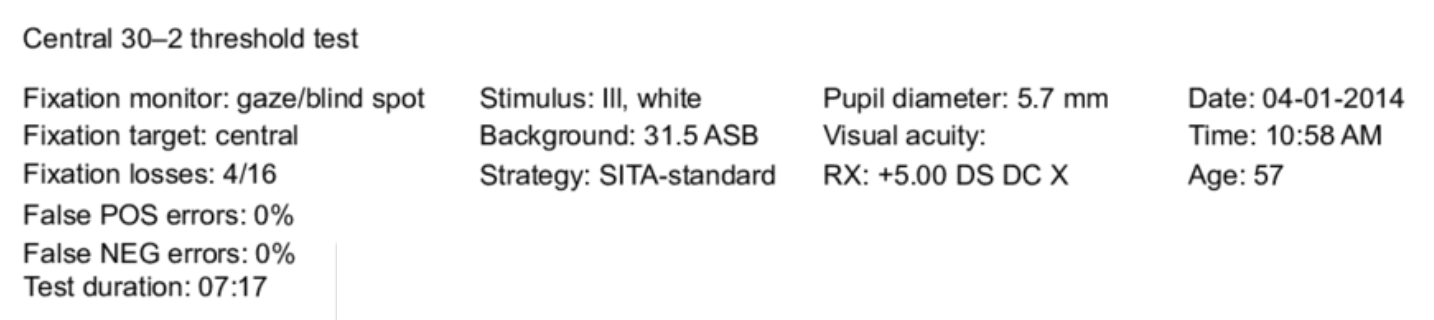
\includegraphics[width=1\linewidth]{images/Sample_Report_Metrics.png}    

    \caption{This figure showcases the standard layout of the test and fixation information found in a HVF report. Retrieved from \citet{HerroLam2015}.
    }

    % use the notation fig:name to cross reference a figure
    \label{fig:example_metrics} 
\end{figure}

This section contain metrics that should not be overlooked by the test provider. False positive/negative rates provide important insight into the validity of the test. A false positive (FP) implies the user has registered seeing a stimulus when there is nothing being displayed. Patients with a high FP are referred to as 'trigger happy' patients as they are clicking when they do not need to. A false negative (FN) is logged when the user does not register a stimulus in a position where they have previously registered a stimulus. Although not absolute, a high false negative rate could imply the user is not paying good attention during the test. Fixation loss is measured by displaying stimuli in the users blind spots throughout the test. If they register a stimulus it is marked as a fixation loss. In Figure \ref{fig:example_metrics} a loss of 4/16 implies out of 16 stimuli displayed in the patients blind spot, 4 were picked up. A fixation loss of more than 20\% indicate a poor reliability of the report \citep{RuiaTripathy2021HVF}

Although published guidelines used to advocate that FP rates of up to 33\% are acceptable although \citet{Heijl2021PerimetryPrimer} found that FP rates of even 5\%  to 10\% significantly affect graphical plots in the report. \citet{Chaglasian2013} a doctor of optometry agrees that accepting a rate of 33\% should not be followed. They further go on to say that a FN result of 10\% to 15\% are more indicative of patient not paying goo attention during the test. Results with FN rates around this value may look worse than the patients visual field actually is.

In figure \ref{fig:example_metrics} both error rates are 0\% indicating that the user paid attention during the test as well as marked any stimuli that was in the same position as a stimulus they marked earlier. The fixation loss in figure \ref{fig:example_metrics} implies this test is likely unreliable as the loss is >20\%. 

\textbf{Test Visualisations and Graphing} \newline
This sections contains a sub selection of graphs that are found on a HVF report. These specific graphs are used to visualise the users response to stimuli as well as compare their responses to the 'norm'. Gray scale plots like \ref{fig:example_gs} are often the most prominent visualisation and therefore other elements of the report can be neglected. \citet{Chauhan2008PracticalRecommendations} state that decision-making based on the examination of gray scale plots should be avoided. Total Deviation graphs are useful for finding localised defects that might be hidden by generalised depressions.
\begin{figure}[htbp]
    \centering
    \begin{subfigure}[b]{0.45\textwidth}
        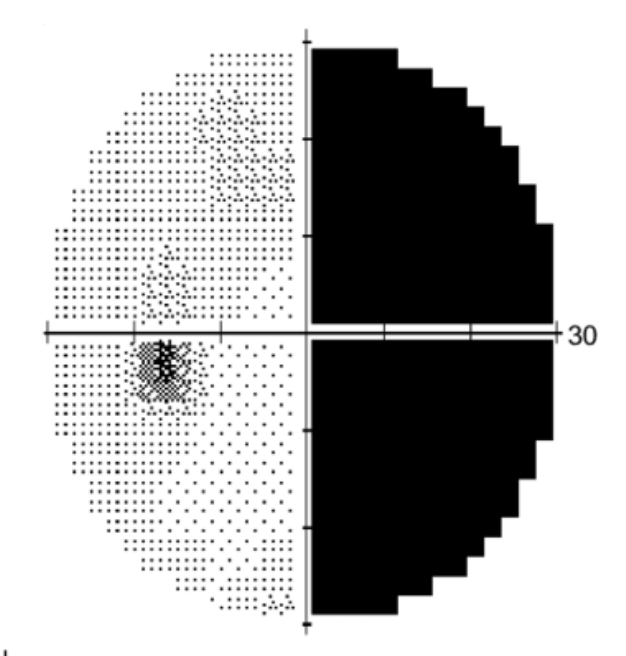
\includegraphics[width=\textwidth]{dissertation/images/Grayscale_Example.png}
        \caption{Gray scale. Showcasing the retinal sensitivity of the patient, with black showcasing a lack of sensation up to white at the other end of the scale}
        \label{fig:example_gs}
    \end{subfigure}
    ~
    \begin{subfigure}[b]{0.45\textwidth}
        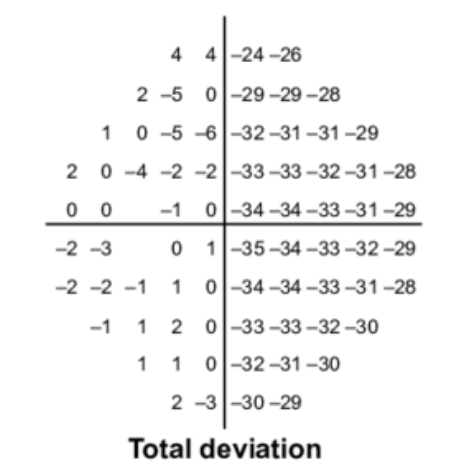
\includegraphics[width=\textwidth]{dissertation/images/Total_Deviation_Example.png}
        \caption{Total deviation of the patients visual field from the normal of their age group}
        \label{fig:example_td}
    \end{subfigure}
    ~   
    \caption{Test report visualisations that display an abnormality in the patients visual field. Figure \subref{fig:example_gs} shows a visual representation of the defects in the users visual field. Figure \subref{fig:example_td}
    shows more quantitative data, comparing the users deviation from the 'norm'. This example showcases a patient who was diagnosed with right-side homonymous hemianopia. Retrieved from \citet{HerroLam2015}.}\label{fig:example_result}
\end{figure}
\newline
Ultimately, the diagnostician uses all visuals included in the report to make an informed decision. Although visuals like the gray scale might attract initial attention, no conclusion can be made on the users attention to the test nor other metrics that can be found in the first part of the report. 




\subsection{Visual Field Testing with Hemianopia} \label{background:VFT_Hemianopia}
The \citet{BIOS2016VisualFieldLoss}  describe Hemianopia as a visual field defect, most commonly caused by strokes, lesions or tumors. Homonymous Hemianopia, the most common type, refers to the complete loss of visual field on the left or right side of the patients view of each eye. Defects of the visual field are typically diagnosed by a method called confrontation, however \citet{Pandit2001VisualFields} demonstrate that confrontation tests have a lower sensitivity compared to automated perimetry. MRI's are the most common diagnostic test for homonymous hemianopia however a complete evaluation of the visual system is recommended, including a visual field test to highlight any visual field defects \citep{NANOS2021HomonymousHemianopia}

\citet{Kedar2011VisualFields} argue, although there are very few clear guidelines for the performance and interpretation of visual fields in neuro-ophthalmic disorders, a visual field test for patients with symptoms serve an important purpose:
\begin{enumerate}
\item \textit{Diagnostic}: Patterns from the visual field defect can help localise the site of the legion
\item \textit{Follow-up}: Visual Fields provide a useful tool to monitor resolution or recurrence
\end{enumerate}

\section{Virtual Reality} \label{background:VR}

Virtual Reality, commonly abbreviated to VR, is a simulated 3-dimensional, computer-generated environment that facilitates interaction between the environment and the user. Interaction with virtual reality could be facilitated by eye-tracking (\ref{eye-tracking}), hand and gesture recognition, voice commands, physical movement and haptic feedback.

In 1965, Ivan Sutherland created the "ultimate display" Head-Mounted Display (HMD) which is often credited as the first instance of a virtual reality headset as we understand it now \citep{VRS2017}. His goal of simulating reality to the point where you could not tell the difference from actual reality is for many virtual reality developers, the ultimate goal of this technology. Presently companies such as HTC, Oculus and Valve continue to develop and commercialise many of Sutherland's principles, allowing VR technology to reach more consumers than ever. According to \citet{Alsop2024} the global virtual reality market seen \$1.7 billion in revenue in 2018 with a projected market revenue of \$11.45 billion in 2028. Although these companies are heavily concentrated within the gaming and entertainment industry, making up x amount according to Y, there is growing interest in using VR in other sectors such as education and healthcare.

However, there are still problems with virtual reality. \citet{HamadJia2022VRChanges} highlight a number of limitations with current virtual reality technology. Firstly, due to the large number of VR manufacturers standardisation is still very limited (\citet{Timmerer2017ImmersiveMedia};\citet{HamadJia2022VRChanges}). The unfortunate consequence of this means applications are not easily transferable among VR suppliers. Furthermore one of the most prominent issues with VR is 'cybersickness'. Cybersickness is a broad term used to describe feelings of nausea, dizziness and light-headedness. Similar to motion sickness these cluster of symptoms are typically caused by a combination of the weight of the headset, lack of synchronisation between the users movements and the headset as well as prolonged VR exposure. 

\subsection{VR in Healthcare}
Virtual reality has seen growing application in the healthcare industry. With proven success in the education sector, VR is now being used in training to simulate medical procedures to clinicians. Furthermore, VR is being used to show patients what to expected during their procedures as well as studies into its use as a rehabilitation factor.

Research shows there is potential for medical checkups to been done in virtual reality. \citet{beyondreality2022} at the national research group concluded 24\% of users in their study would be willing to attend a medical check-up in VR. Another study by \citet{Winter2021} trialed using head-mounted displays (HMDs)  on multiple-sclerosis and stroke patients during their study to see if it would improve their recovery. Using traditional treadmill therapies, patients were given a HMD to wear during their training. 71\% of patients and 89\% of healthy participants preferred using a HMD, with both groups having a higher walking speed when using the HMD. Furthermore no cybersickness was reported. They concluded that in this instance using VR would be helpful in improving training motivation. Conversely on the clinical side, \citet{Samadbeik2018ApplicationsVR} found that there was a higher accuracy in medical practise by people trained in VR in 87\% of studies they reviewed. Another study, and the first of its kind, on a patient with homonymous hemianopia and another with bitemporal hemianopia found both users visual field (measured by binocular Esterman and monocular Humphrey full-field analyses) improved after six-seven weeks of 15 minute sessions of audiovisual simulation every two days. They concluded that home-based virtual reality visual rehabilitation was feasible in real world conditions and such technology was effective on improving visual quality and quality of life.

\subsection{Eye Tracking} \label{eye-tracking}
Eye tracking is a form of interaction between the computer-generated virtual reality and the user. Eye tracking makes use of infrared sensors built into the HMD to capture the pupil and direction of where the user is looking. It makes use of the distance between the users pupil and cornea to evaluate where the users gaze lies.

Eye tracking has been a particularly exciting advancement for researchers as it allows a deeper understanding of user behaviour. By analysing where a users focus is and for how long, researchers can improve VR experiences and gain insights into cognitive process \citep{Farnsworth2022VREyeTracking}. In educational and therapeutic settings researchers are able to understand users engagement. Its functionality also allows for gaze-based interaction, that is, where users can control their virtual reality experience by interacting with the environment using their gaze. Programs can use data collected from the HMD to update their environment in real time.

However, eye tracking must be precise and reliable in order for it to be utilised effectively in real world applications. This is especially important in healthcare, where data from eye tracking might influence treatment of a patient. \citet{SchuetzFiehler2022} concluded the HTC Vive Pro Eye to be highly reliable in its calibration and measurements, and within its stated device specifications. Although the eye tracking calibration software was found to be accurate, when using the eye tracking software on users with glasses both precision and accuracy were found to be significantly reduced. Furthermore, regardless of whether the user was wearing vision correction, gaze accuracy and precision was found to be highest in the centre of field of view while decreasing as the user looked to their periphery. 

\subsection{Visual Feedback}
Visual feedback is an important aspect in user interfaces (UI). It enhances interaction and immersion by providing a response to user actions or behaviours. By communicating to the user through visual queues, the user knows their action has been recognised by the system. Feedback to the user can range from simple colour changes in elements of the UI to complex animations that guide the user through a process.

The effectiveness of visual feedback has been extensively researched, particularly in the field of human-computer interaction (HCI) where there is a focus on usability and user experience. Studies have shown that well-designed visual feedback can improve task performance, reduce errors and increase user satisfaction \citep{HCIMotionDesign2023}. \citet{HCIMotionDesign2023} goes on to emphasise the importance of immediate user feedback, noting that it keeps users informed on the outcome of their interactions, which in turn enhances the overall usability of a system.

In VR applications, visual feedback can be even more crucial due to the immersive nature of these environments. Users rely heavily on visual queues and prompts outputted by the system when navigating and interacting with the system. Furthermore research found that motion and visual design impacted users emotions and perceived usability \citep{Hassenzahl2008}. Another study by \citet{Gibbs2022Visual} found visual feedback alone gave a greater sense of presence that haptic feedback alone.

However, if implementing visual feedback in a VR application or in a wider sense, any application, visual feedback must consider various factors to ensure effectiveness. We need to adapt visual feedback to accommodate different users, such as those with visual impairments \citep{HCIMotionDesign2023}. This can be done by using contrasting colours, adjusting sizes and animation speeds. Furthermore its important that a feedback system remains informative whilst not obstructing the user from completing their primary action, such might be the case where there are multiple sources of visual feedback that could overwhelm the user.


\subsection{Visual Field Testing in VR}
There have been a number of prior attempts to conduct a visual field test within VR. One such attempt by \citet{Stapelfeldt2021VRGlaucoma} used an Oculus Quest with the game engine Unity to design a custom VR application to test a users visual field. They collected results from 114 participants over 12 months, testing them on both a Octopus 900\footnote{Widely used automated perimetry device used within ophthalmology.} and their custom VR system. They compared patients mean defect (average deviation of measured visual field from normal values) from both systems. They were interested in seeing if this VR system was non-inferior to the benchmark Oculus 900, and the researchers concluded their custom VR perimetry test performed comparably to a clinically performed AP test in healthy and early/moderately affected glaucoma patients.

Another implementation by \citet{Wroblewski2014TestingVisualField}, called VirtualEye, used a HMD and eye tracking to assess a users VF using automated perimetry. They used two modes of interaction, a standard use of response by clicking on a mouse, and more uniquely a visual grasp, where eye tracking senses a change is the users gaze direction and uses this as evidence of target acquisition. It is capable of doing a full 24-2 threshold test. A point-by-point comparison between the different systems indicated that there was minimal systematic difference. However, there was a systematic shift of 4-6dB in the results from VirtualEye compared to results from the HVF analyser, especially in higher dB ranges. This indicates that VirtualEye recorded lower sensitivity measurements. However their usability survey did indicate patients generally accepted the HMD. They concluded that this research appears to validate the concept of a HMD perimeter test (including visual grasp).

\section{Chapter Summary}
This chapter provided an overview on two main areas of research relevant to this project, visual field testing and virtual reality (VR).

Under Visual Field Testing, we delved into the evolution of this diagnostic tool, starting with the first documented visual field testing by Hippocrates. We progressed through the advancements of Automated Perimetry and finally detailing the significance of the Humphreys Visual Field (HVF) test. We outlined the protocol and typical results obtained from testing, along with exploring the challenges associated with current testing methods. Finally we explained Hemianopia as a condition and emphasised the importance of Visual Field Testing for individuals with neuro-ophthalmological conditions.

Moving to Virtual Reality, we discussed the promising results that Virtual Reality is getting as it emerges in the healthcare industry. We discussed the importance of eye-tracking technology in enhancing virtual reality, and explored research regarding the concept of real-time visual feedback to a user. Finally, we looked at past work exploring visual field testing in virtual reality. Papers from \citet{Stapelfeldt2021VRGlaucoma} and \cite{Wroblewski2014TestingVisualField} showed us that there is a potential for successful application in this area of research.

Our background aims to provide the context and groundwork to understand our motivations and objectives of this research project. By understanding the evolution of visual field testing and the emerging role of virtual reality in healthcare, we aim to highlight the potential applications in this area of research. Furthermore, keeping current VR technology in mind as well as the current challenges faced in visual field testing, we can use this information to steer our projects requirements.


%============================4-======================================================================================================
\chapter{Analysis and Requirements}
\section{Problem Specification}
The aim of this project was to assess whether real-time visual feedback during testing could enhance the effectiveness of our visual field test in virtual reality, while also evaluating its usability. Effectiveness could be measured using fixation loss, false positives and false negatives found in a typical Humphrey Visual Field (HVF) test report (the validity metrics mentioned in \ref{validty-metrics}). To our knowledge, there has been no project that has provided real-time visual feedback to the user during the testing process. This feedback would indicate whether a user was looking at the designated stimulus, in this instance, the centre, by altering the colour of said designated stimulus. It was hypothesised that this feedback could be achieved by using the results of eye-tracking software to alert the user when their gaze shifted from the central point during testing. By comparing the group that receives real-time feedback on their gaze with participants who do not, there may be an observable difference in effectiveness. Furthermore, by collating and analysing user evaluations through surveys and performance metrics the usability (encompassing clarity, comfort and user experience) of this feature could be analysed. The user study will be comprised of eight healthy individuals with no diagnosed neuro-ophthalmology conditions plus one individual study of a user with right-side homonymous hemianopia to understand the usability and effectiveness of this test in patients with visual impairments while adhering to the ethical principles laid out by the school of computing science.

\subsection{Functional Requirements}
This project should satisfy the following functional requirements as listed below:
\begin{itemize}
    \item The program must provide immediate visual feedback based on the eye-tracking data collected during the programs runtime. Users must be alerted if their gaze shifts from the designated focal point.
    \item Test parameters such as stimulus location, display time, and size must be customisable to accommodate different tests.
    \begin{itemize}
        \item The program should read stimulus location data from a text file 
        \item Stimulus presentation (colour, size and shape should be assigned in  the environment).
    \end{itemize}
    \item Stimuli should be displayed on a specified 'canvas', this would allow for future work to include background light level dependent on the selected canvas.
    \item The system must register user responses to stimuli using a controller. It should accurately record which stimuli are acknowledged by the user.
    \item Eye tracking should be initiated at the start of a test, continuously monitoring the users gaze through the test duration.
    \item At the conclusion of a test, the program should log details about stimuli presented and whether the user has detected them. This includes timestamps, whether the user is looking at centre and whether it was accurately acknowledged. 
    \item Once any logs are finalised, the program should use the collected raw data and convert them to visual representations. This includes:
    \begin{itemize}
        \item A gray scale image
        \item A heat map of user gaze
    \end{itemize}
    \item Finally, once graphical visualisations have been created the final script should be called to write visualisations and raw data metrics to a pdf report, similar to a HVF report. 
    \item Data should be structured in a repeatable way so test reports are comparable
    
    \item A number of raw data points should be collected during the test:
    \begin{itemize}
        \item The coordinates of the users gaze 
        \item The stimuli being displayed and whether the user records there presence
        \item The duration of the test
    \end{itemize}
\end{itemize}

\subsection{Non-Functional Requirements}
\begin{itemize}
    \item The program should be usable after a small brief, it should not take long to inform users of the tests workings as control, as the test should not be significantly longer than a standard HVF test.
    \item The systems must ensure repeatability in its outputs, that is, when a user performs the same test multiple times under consistent conditions, the variance in test results should be minimal (if we discount user fatigue). In other words, inter-test variability should be low. If the system is generating accurate and dependable results the system should be reliable 
    \item The system should be usable to a number of users with visual impairments (beyond the scope of visual field testing), such as colour blindness compatibility.
\end{itemize}
\section{Chapter Summary}
In this chapter, we have laid a foundation for this project which is to explore the effectiveness of visual field testing which integrates real-time visual feedback. Recognising a gap in current test practises - where there was no existing methodology that offers real-time visual feedback to the user - our aim is to investigate the potential for such feedback, facilitated by eye-tracking technology, to improve test effectiveness and user experience. We hypothesise that alerting users to unintentional gaze shifts can reduce common validity metrics issues like fixation loss, false positives and false negatives - thereby enhancing the overall reliability of a visual field test.

To achieve this, we have detailed a set of functional requirements necessary for the development of the system. These include capabilities for immediate visual feedback based on eye-tracking data, customise test parameters to accommodate various testing methods, functionality to record accurate user responses, data logging for further analysis and test report generation using visual representations found in standard HVF test reports.
Additional non-functional requirements were highlighted. These include ensuring the system is intuitively usable with minimal instruction as well as maintain repeatability and reliability in test outputs to ensure consistency across multiple tests. Furthermore the system should be designed to be accessible to users with visual impairments to broaden its applicability and inclusively.

By addressing these requirements, this project aims to demonstrate the feasibility and effectiveness of incorporating real-time visual feedback into visual field tests. The design and implementation will follow the objectives and requirements outlined in this chapter, enabling the solution to be developed and later evaluated.

%==================================================================================================================================
\chapter{Design}
\section{Overview} \label{design_overview}
The design of this system can be split into the following sections: Overview, Visual Field Test (\ref{design-vft}), Controller Interaction (\ref{controller-ui}), Eye Tracking Feedback (\ref{eye-tracking-ui}) and Report Workflow (\ref{design-wf}). From the beginning of the project it was clear each section of testing should be abstracted into separate parts, allowing for each section to be changed iteratively when required and also so that one part of the program would not become too complex, or handle too many different requirements. This format also allows for future changes to be made without affecting other sections of the program.
\begin{figure}[htbp]
    \centering
    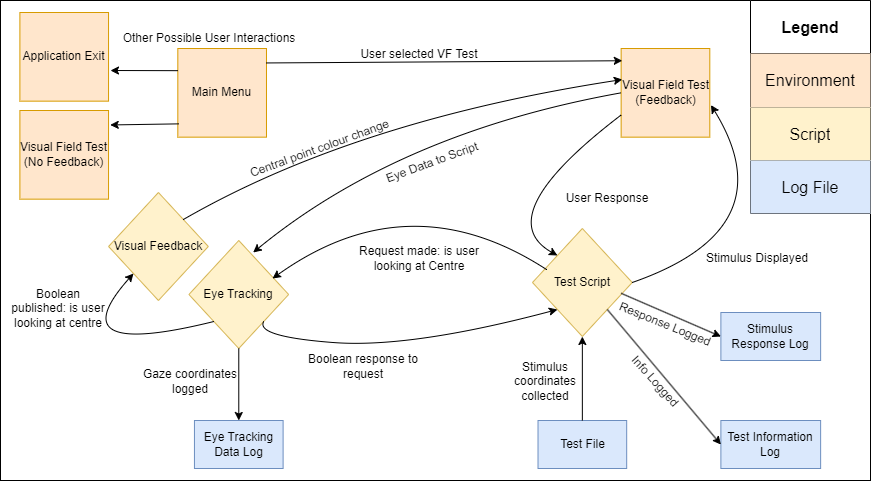
\includegraphics[width=1\linewidth]{dissertation/images/Design_Overview.png}    

    \caption{A high level diagram to show an overview of the design of the project, where arrows represent an action either by the user or the system. A square represents a state, and a diamond represents a script. 
    }
    \label{fig:Design_Overview} 
\end{figure}
\newline
Above, figure \ref{fig:Design_Overview} showcases the high-level design of the program. Initially the user will be in the 'Main Menu' state, from here they can exit, or continue to one of two other states. In this figure the user continues to the visual field test with visual feedback. User data is collected and outputted identically in both testing environments however the main difference between this state and the test without visual feedback is the inclusion of the visual feedback script. This is what updates the central point depending on the input it receives. Most scripts interact with the test script, therefore the test script can be thought of as the 'Main' function in this system. Its important to note the dependencies in the above figure. 

In this design there are the following dependencies:
\begin{itemize}
    \item \textbf{Test Script} depends on:
    \begin{itemize}
        \item The inclusion of a Test File input
        \item Eye Tracking Script
    \end{itemize}
    \item \textbf{Eye Tracking} depends on:
    \begin{itemize}
        \item Visual Feedback Script
        \item Test Script
    \end{itemize}
    \item \textbf{Visual Feedback} depends on:
    \begin{itemize}
        \item Eye Tracking Script
    \end{itemize}
\end{itemize}

Understanding the diagram in figure \ref{fig:Design_Overview} (the 'big picture') and keeping note of the dependencies between each part of the program means we can now delve into more detail about each section of the design.

\section{Visual Field Test} \label{design-vft}
The actual test aspect of this program can be thought of in three distinct parts. Firstly, is the environment in which the user is placed. This is the visual part of the program and where testing would be conducted on the user. In order to facilitate the testing, the system requires the utility to process test files, display them to the user in the environment and then record the users results - this utility is made up in the testing script and is thus the second part. Finally is the the input. The test needs some sort of instruction. A test file should contain the necessary instructions for the system to run effectively. 

These three parts encompass most of the necessary functional required to run a test however, notably, interaction is handled separately. Furthermore as the test runs automatically once it begins there should not be any inherent need for the test operator to intervene. 

\begin{itemize}
    \item \textbf{Environment}
The environment has the flexibility to be formatted with different shapes or background colour so long as it is linked to the testing function. As described earlier it is the visual part of the system. Within the visual field test it displays the stimuli and testing field. Furthermore, it shows the central fixation point throughout the program, and is what connects the back-end of the program with the user.
    \item \textbf{Testing}
The testing script is what handles sending stimuli to the environment. It reads in an input, and then begins with the test. 
It displays the stimulus to the designated environment and listens for a user response. When a user responds to seeing a stimulus, their response is logged. As mentioned in the Overview {\ref{design_overview}} the testing script interacts with eye tracking to log whether the user is looking at the designated central point. It does so by sending a request to eye tracking, which in turn responds with the appropriate boolean response. Finally, when all stimuli are displayed the testing script produces logs on the type of test performed as well as the users responses. 
    \item \textbf{Input}
The input contains information on the points to be shown during testing. It should be read in by the testing script and its data stored. It could contain data such as the position of the stimulus or time it should be shown for.
\end{itemize}
Below is Algorithm \ref{alg:visual_field_testing}. This is a pseudocode outline of the testing script. As we can see it makes reference to a Canvas (our \textbf{Environment}) and a Test File (our \textbf{Input}). Fundamentally, it reads in our stimuli, iterates through them, and displays them accordingly. The program waits for a user input (for a predetermined time outlined in the test file input). If the user triggers and is looking at the centre (determined by making a call to the eye tracking node), if the user identifies the stimulus but is not looking at the centre, it is logged accordingly. Finally the program records either a missed response or a false positive if they click when nothing is there. This data is outputted to be used in the report workflow (section \ref{design-wf}).
\newline
\begin{algorithm}[h!]
\caption{Visual Field Testing Algorithm}
\label{alg:visual_field_testing}

\KwIn{Test File containing number of stimuli, response time, and stimulus positions}
\KwOut{Log files for results, false positives, and test info}

\tcc{Setup initial references and start test}
Reference \textbf{Canvas}\;
Reference \textbf{Eye-Tracking}\;
Start Test and Record Start Time\;
Setup File Paths for Logging Output\;

\tcc{Read Test File and parse parameters}
Read Test File: Parse Number of Stimuli, Response Time, and Stimulus Positions\;
Setup Writers for Results, False Positives, and Test Info\;

\tcc{Main loop for displaying stimuli and logging results}
\ForEach{Stimulus}{
    Display Stimulus at Current Position on \textbf{Canvas}\;
    Wait for Trigger\;
    \eIf{Triggered Within Response Time \textbf{and} Looking at Centre}{
        Log True for Response\;
        Log True for Looking at Centre\;
        Log Reaction Time\;
    }{
        \eIf{Triggered Within Response Time \textbf{and} Not Looking at Centre}{
            Log True for Response\;
            Log False for Looking at Centre\;
            Log Reaction Time\;
        }{
            Log Missed Response\;
        }
    }
    Wait Random Interval Before Next Stimulus\;
    \If{Trigger During Waiting}{
        Log False Positive\;
    }
}

\tcc{Clean-up Logging}
Stop \textbf{Eye-Tracking} Script\;
Log Results for Each Stimulus and False Positive\;
Close Writers\;
Close All Open Files on Application Quit or Disable\;

\end{algorithm}



Finally although interaction is covered in the next two sections, below is a short overview of how the visual field script should use controller and gaze data. The user will have two methods of interaction with the testing script, using their controller (section \ref{controller-ui}), or implicitly\footnote{Implicit interaction: without the behest or awareness of the user \citep{JuLeifer2006ImplicitInteractions}} using their gaze (section \ref{eye-tracking-ui}). Controller interaction is used to communicate to the system that you have identified a stimulus. Gaze data is used in conjunction with the eye tracking script to log the correct information in the output of the testing script.

\section{User Interaction} \label{controller-ui}
In order for system to work there needs to be a way for the user to inform the system when they want to transition to another environment, begin the test, or communicate to the system that they have identified a stimulus. In Virtual Reality programs this is commonly achieved with a controller. This device typically composes of buttons, triggers, thumb-sticks or other sensors. Therefore there needs to be a framework in place that can translate real-world user actions into actions performed in the virtual environment. In this design that framework would need to be implemented between the visual field test environment and the test script. It would enable many of the necessary features that would satisfy the outlined functional-requirements. 
\section{Eye Tracking Feedback} \label{eye-tracking-ui}
The eye tracking and visual feedback components make this section of the design fairly difficult due to their many dependencies and their inclusion of many of components we have discussed earlier. As we have highlighted above in the overview (\ref{design_overview}) both components comprise of the visual field test environment and a mechanism to identify if the user is looking at the centre. This further requires a mechanism to provide the feedback to the environment. Finally a response to the test script every time it requests 'is user looking at the centre?' needs to be facilitated.
We can break this section into two parts:
\begin{itemize}
    \item Visual feedback in this instance is the changing state of the central fixation point. This point can present as different colours depending on where the user is looking. The visual feedback relies on the eye tracking data collected by a HMD, which in turn allows for the alteration of the visual field testing environment where the central point resides.

    \item Eye tracking takes data from the users gaze. This needs to be done frequently as so collected data can be distributed to the visual feedback node in real time to ensure the visual feedback is correct. Furthermore, we have already established any eye tracking that is implemented must feedback to the test script so we can ensure our validity metrics are recorded.
\end{itemize}
\section{Report Workflow} \label{design-wf}
Finally in our design we need to understand how our raw output files can be generated into a PDF report. This is done by a separate node called at the end of the test script. In turn this node follows the workflow highlighted below in figure \ref{fig:Design_Workflow}. 
In this figure we see an abstraction of the design of this system. When the user is in our test environment and our test script has completed, we see a number of nodes be called. Fundamentally this part of the design is about turning our raw data files from earlier, into processed data which we can then turn into our final report.

Processed data can be thought of as data that has been created using raw data. Raw data is comprised of the output from the test script and the eye tracking script. We use these outputs to make our metrics and visuals, which in turn is formatted into a report. All data processing scripts are handled by our data processing script, which is embedded in our project. The Metrics, Graphing and PDF Generation script are called from within the project but are not actually directly attached in this layout. This allows the flexibility of test operators to call these scripts on any raw data, instead of relying solely on the program to run its course before the scripts are called.
\newpage \begin{figure}[htbp]
    \centering
    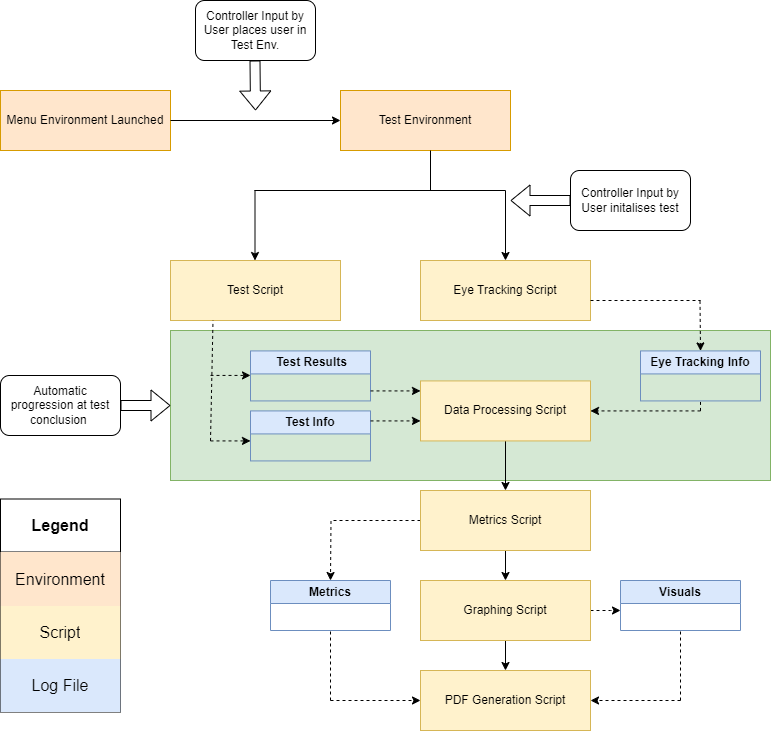
\includegraphics[width=1\linewidth]{dissertation/images/Design_Workflow.png}    

    \caption{A high level diagram to show an overview of the design of the project, where arrows represent an action either by the user or the system. A square represents a state, and a diamond represents a script. 
    }

    \label{fig:Design_Workflow} 
\end{figure}
Finally the design of the actual report needs to be discussed. Our report needs to be grounded in the industry norm we introduced in our background (\ref{Background-HVF-Results}). For this reason you can see a side-by-side comparison of a typical HVF report and our report wireframe in figure \ref{fig:HVF_Report_Wireframe} the initial wireframes of the reports are not dis-similar from a typical HVF report. 

They share a number of characteristics. For instance, the mean deviation and gray scale graph are used in both. Furthermore, testing information is shown at the top. Where our design diverges is with the heat map of the user gaze as well as the user metrics. User metrics will give the reader a quick summary of important information such as time looked at the centre, reaction time and further metrics. The heat map will allow test operators to see where the user looked during the procedure.
\newpage \begin{figure}[htbp]
    \centering
    \begin{subfigure}[b]{0.49\textwidth}
        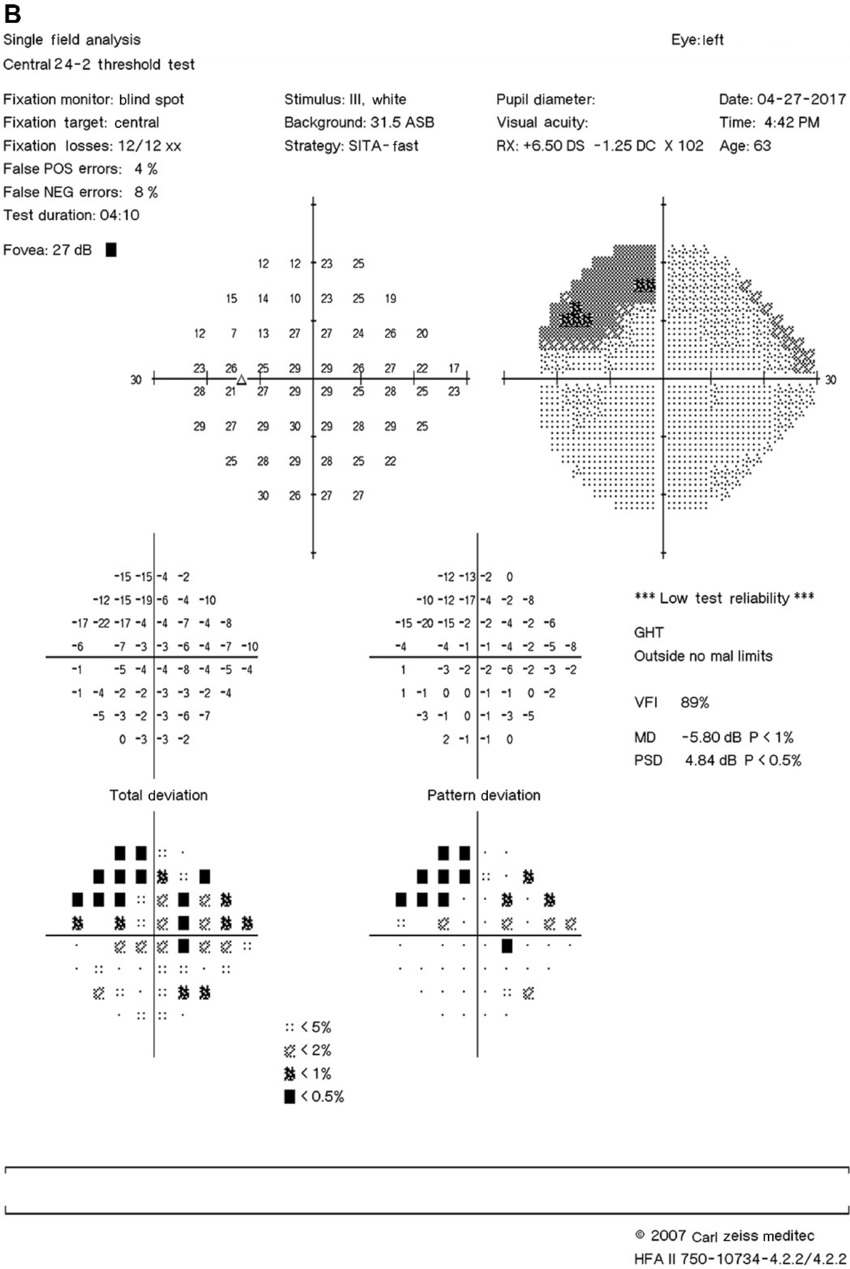
\includegraphics[width=\textwidth]{dissertation/images/HVF-Report-Full.png}
        \caption{Standard HVF Test Report. Retrieved from \citet{Vercio2019}.}
        \label{fig:HVF_REPORT}
    \end{subfigure}
    ~
    \begin{subfigure}[b]{0.49\textwidth}
        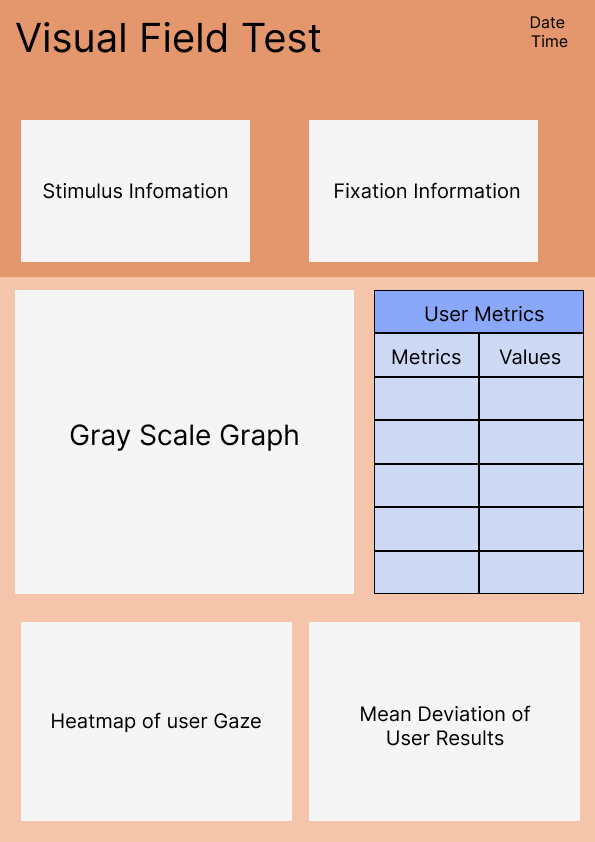
\includegraphics[width=\textwidth]{dissertation/images/Report_Wireframe.png}
        \caption{Initial wireframe design of test report.}
        \label{fig:REPORT_WIREFRAME}
    \end{subfigure}
    ~  
    \caption{Contrasting the two images there are similarities between both reports. \subref{fig:REPORT_WIREFRAME} shares various characteristics with the standard HVF report in \subref{fig:HVF_REPORT}. Gray scale graphs, mean deviation and test information (located at the top) are included in both reports.}\label{fig:HVF_Report_Wireframe}
\end{figure}
\section{Chapter Summary}
In this chapter we have discussed an abstraction of our implementation. Our design covers the key areas of our project, from its general layout, each parts dependencies and then the workflow an implementation would need to follow. We have discussed how our visual field testing algorithm would function. Furthermore we have covered the interactions that would need to be facilitated between each area as well as how our usesr would interact explicitly and implicitly with the system. Finally we displayed a prototype wireframe of how our results should be formatted and displayed to the user in an implementation in line with research we laid out in our background. In the next chapter we will cover the hardware, software, scripting and Software Development Kits (SDKs) as well as the design we outlined above to implement our project.


%==================================================================================================================================
\chapter{Implementation}
\section{Overview}
This chapter will delineate the hardware, languages and environments that were used in conjunction to create the system. It follows a similar structure of the previous design chapter so the reader can understand how it has influenced this implementation. It must be noted, although they divulge, sections \ref{hardware}, \ref{unity} and \ref{SteamVR} have a similar structure to \citet{russell2023} as he was a fellow student using the same VR setup, and therefore there are some similarities in these referenced sections. 

Finally to view the source files of this projects implementation, please review \ref{appendix:source_files}.
\section{Hardware} \label{hardware}
The virtual reality hardware used in this implementation was the HTC Vive Pro Eye\footnote{https://developer.vive.com/resources/hardware-guides/vive-pro-eye-specs-user-guide/}. This was of great benefit due to its inbuilt eye tracking technology that could be used later for the visual feedback based on the users gaze. Furthermore, the HMD comes with two tracked controllers which was used to facilitate user interaction. The headset advertises a trackable field of view (FOV) of $110^\circ$ for eye-tracking with an accuracy of $0.5^\circ - 1.1^\circ$ (within FOV $20^\circ$). It outputs user gaze data at a frequency of 120Hz. Finally the headset uses two separate OLED displays, one for each eye. This serves as a viewpoint for each respective eye and creates a stereoscopic effect that provides depth perception. The headset operates with two external base stations setup around the room. These base stations emit infrared light to track users precisely.
\begin{figure}[htbp]
    \centering
    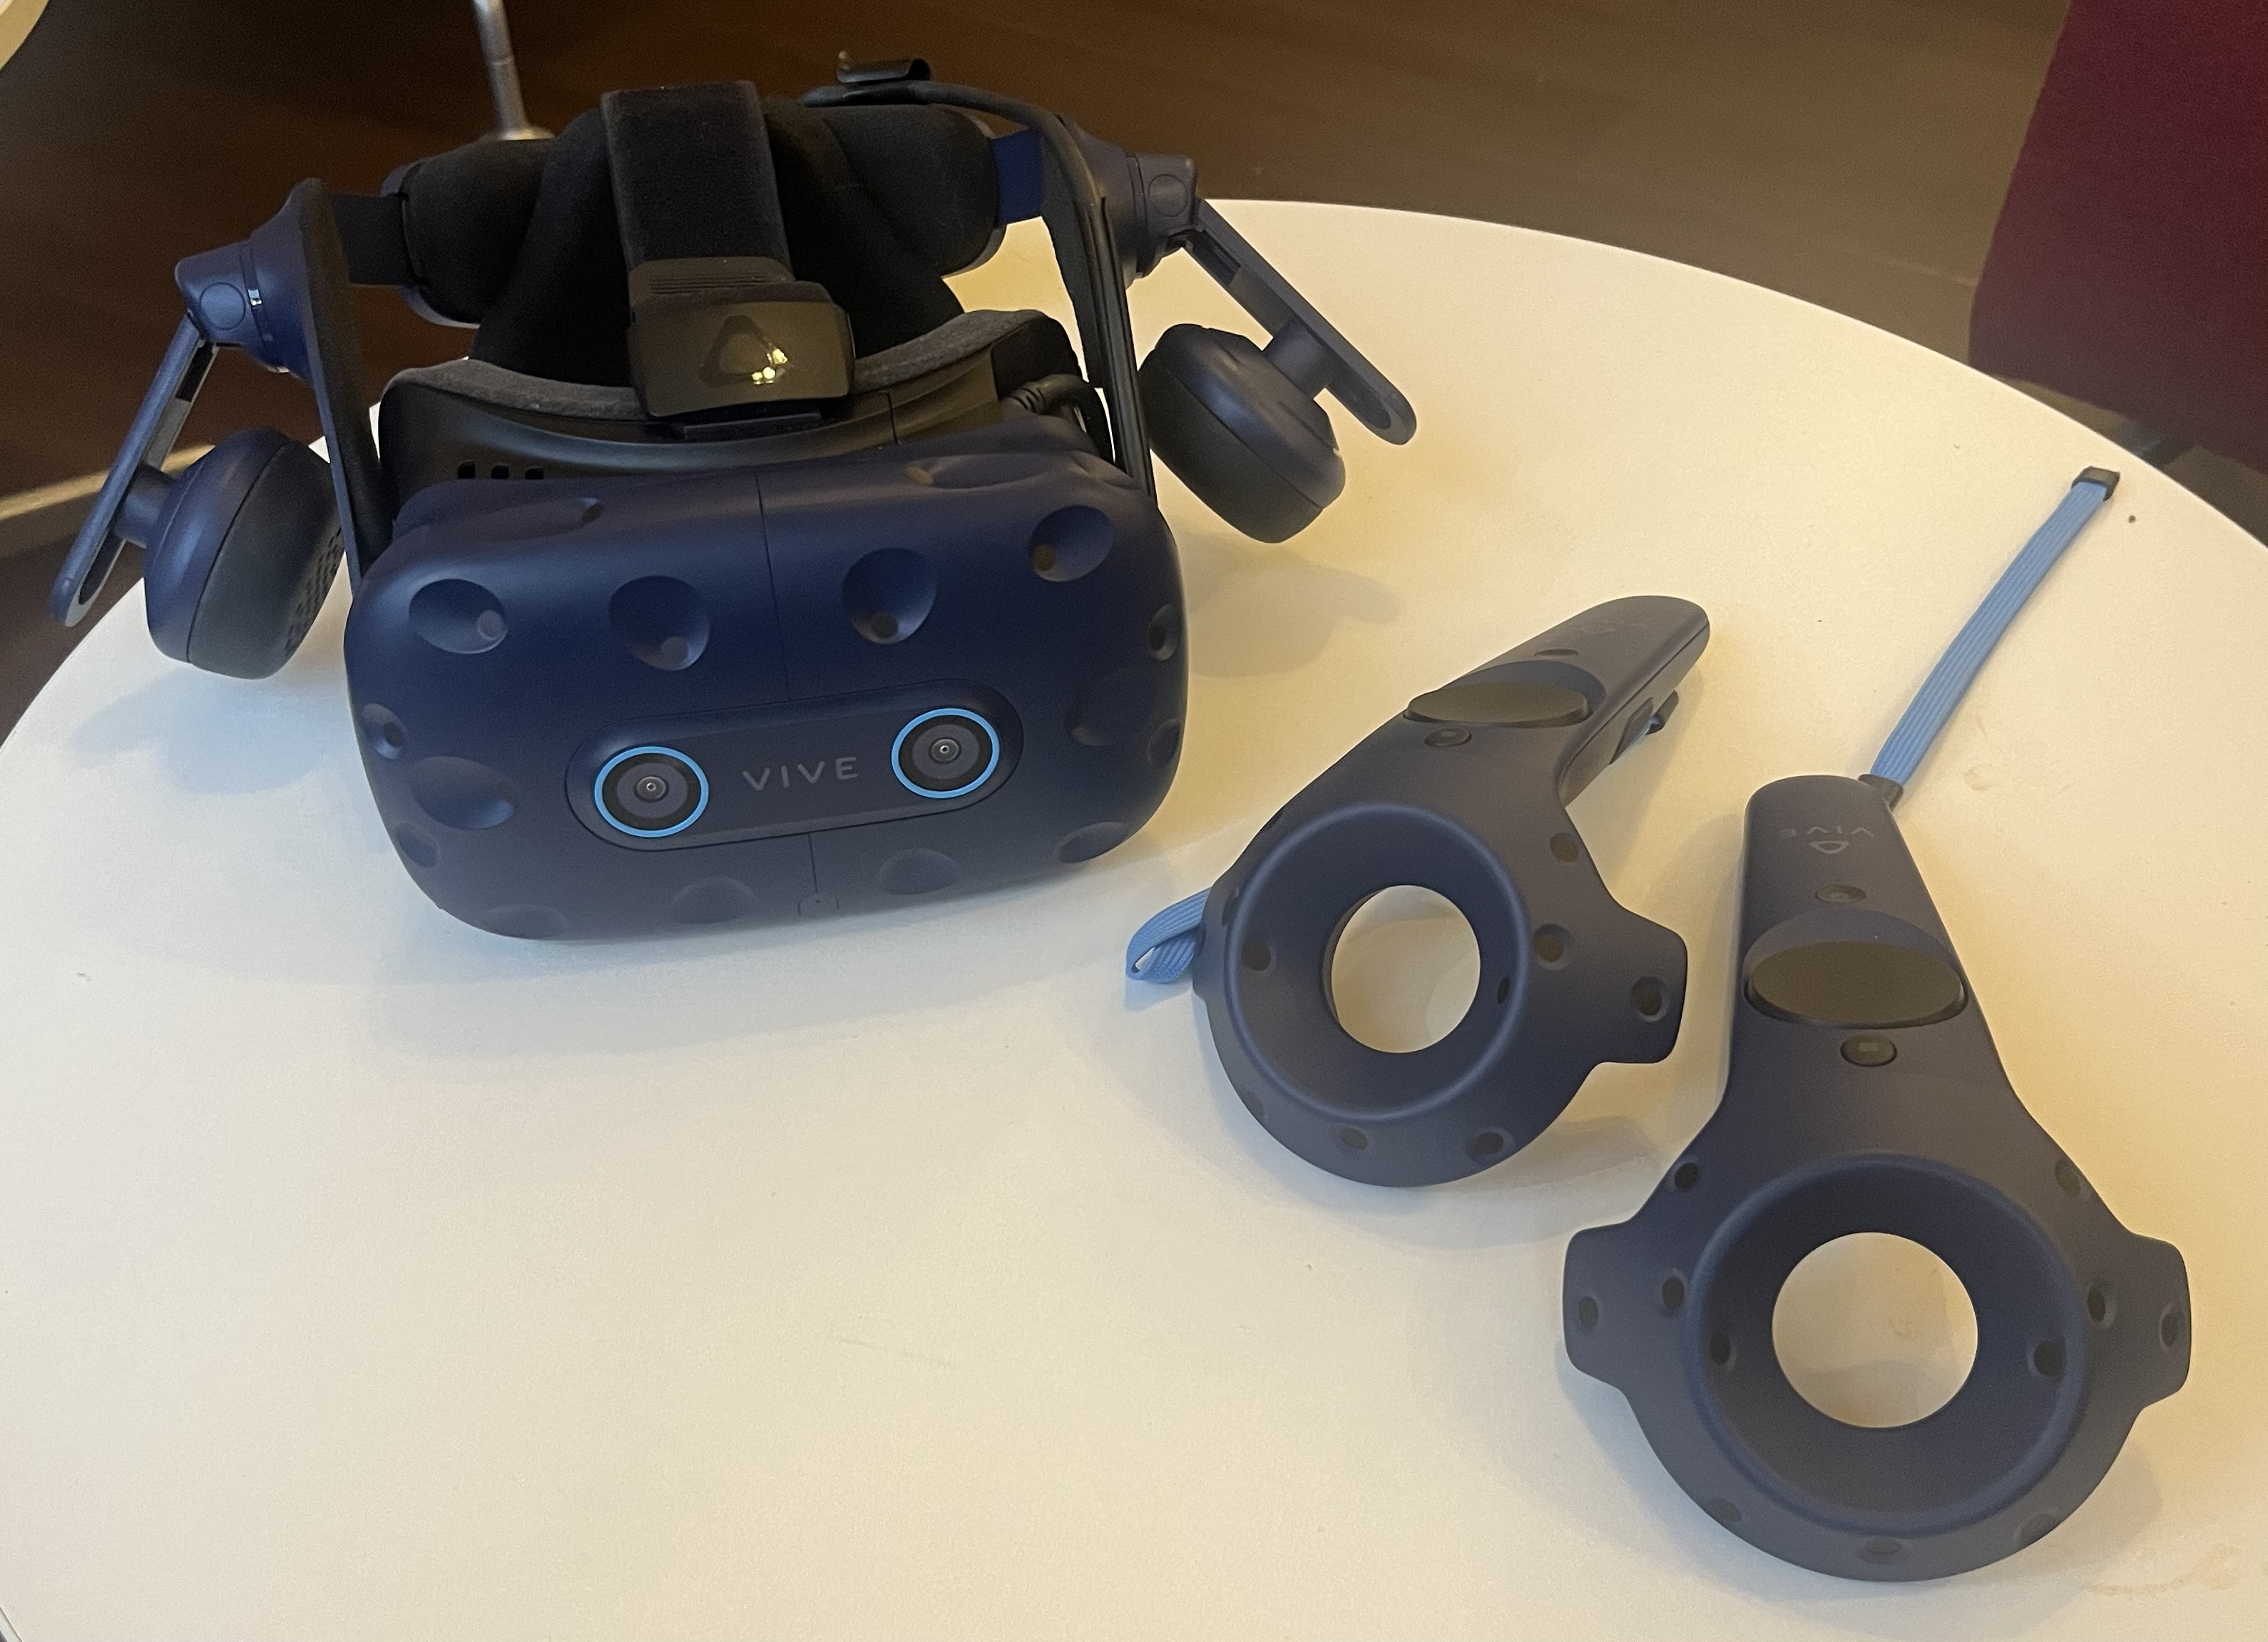
\includegraphics[width=0.6\linewidth]{dissertation/images/HTC_Headset.jpg}    

    \caption{The HTC Vive Pro Eye Headset used in this implementation. Beside the HMD is the pair of wireless controllers that are used by the user to interact with the program.
    }
    \label{fig:HTC_Headset} 
\end{figure}

\section{Virtual Reality Environment}
\subsection{Unity} \label{unity}
Unity is a cross-platform game engine that is used in game-development, 2D and 3D modelling and extensively in VR development. This engine was chosen because of its support for VR, and specifically, for its support of the HTC HMD. In this implementation due to the requirements of SteamVR (\ref{SteamVR}) and SRanipal (\ref{SRAnpial}) Unity version 2019.f.35f1 was selected. Unity is hierarchical, meaning each object in the current scene is attached to the scene or an object that is (this can be several layers deep). All logic is handled by scripts written in C\# that can be copied and attached to an object within their respective scenes. This allows for scripts to be standardised over the entire Unity environment and means other than some minor changes, testing with or without feedback is similarly implemented. 

In order to facilitate interaction between the user, HMD and the Unity environment certain packages were selected to perform these interactions. Although Unity has native VR support using OpenXR\footnote{https://docs.unity3d.com/Packages/com.unity.xr.openxr@1.10/manual/index.html} to support a variety of headsets, we used the SteamVR package for interaction due to its ability to easily access inputs from the HTC controller in scripts. The Unity project has a fairly complex structure due to the number of additional assets that have been imported from the packages and software development kits mentioned below.
\begin{figure}[htbp]
    \centering
    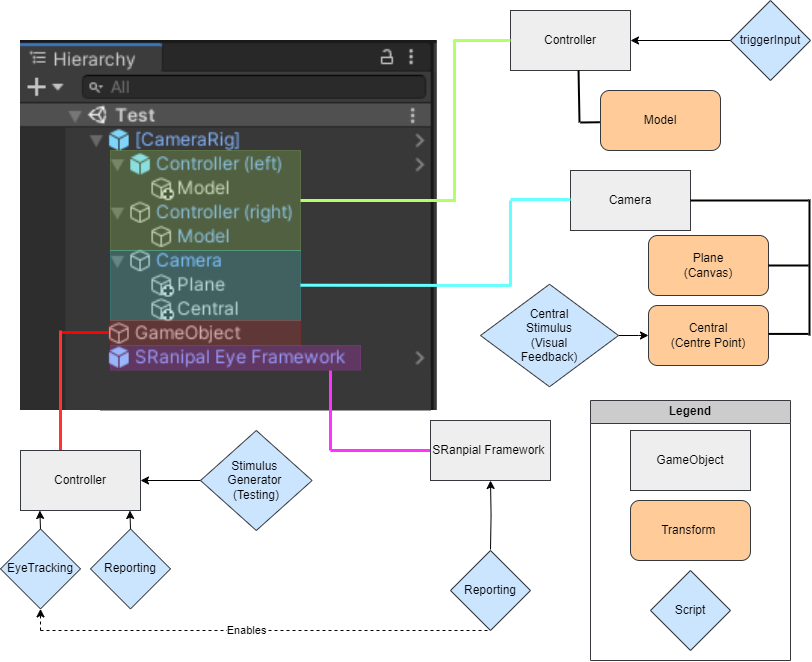
\includegraphics[width=0.7\linewidth]{dissertation/images/Unity_Structure.png}    

    \caption{A labelled diagram of our projects Unity structure. Detailing GameObjects, Scripts and Transforms.}
    \label{fig:Unity_Structure} 
\end{figure}
\newline
Figure \ref{fig:Unity_Structure} showcases a labeled diagram of the testing scene with feedback. As we can see by the legend the diagram is split into three parts. The light-gray boxes represent a gameObject. GameObjects act as containers for components, the implementation of logic within the environment. As mentioned previously and as  we can see Unity is hierarchical, where gameObjects are held within a scene (in this case \textbf{Test}), and a gameObject has components attached to it - whether that be a Transform\footnote{Position, Rotation and Scale of an object.} or a script that defines behaviour, interaction, or functionalities for the gameObject or wider program. 

\subsection{MonoBehaviour}
MonoBehaviour is a the 'base' class in Unity, the class for which every other Unity class derives its behaviour from. Any script that needs to be within a scene, such as the testing scene must be attached to a gameObject to function and interact with the scene properly. To enable this interaction we need to inherit this MonoBehaviour class to all C\# scripts that are used within our main, test and testing without visual feedback scenes.  Therefore all scripts in this project that are written in C\# inherit MonoBehaviour due to this behaviour and Unity's component-based architecture\footnote{The idea of composing gameObjects by attaching and combining reusable components.}. By using this base class we gain access to a number of useful functions that allow us to add behaviour and functionality to gameObjects. Below is the list of functions we have inherited from MonoBehaviour and used in this implementation: 
\begin{itemize}
    \item \textbf{Awake()}: This function is called when the script instance is being loaded. We use this to setup any references that start may use. In our case we use this to ensure that our interaction buttons are defined before the script starts, to ensure that user inputs are recorded properly
    \item \textbf{Start()}: This function is called on the first frame when the after the script is initialised. It is always called before the update function is called for the first time. We use this to initialise any components that need to be referenced before they are called within update.
    \item \textbf{Update()}: One of the most important functions inherited from MonoBehaviour in each script. This function is called every frame. It is essential for any continuous processes such as checking to see if users have interacted with the controller, measuring and recording the users gaze data and checking to make sure all SDK frameworks are functioning as intended. Update() tends to include the logic in our tracking scripts such as Eyetracking.cs. Furthermore the amount of times \textbf{Update()} is called depends entirely on the time the program  run time and frames-per-second the environment is running at, so each program may call \textbf{Update()} a unique number of times.
    \item \textbf{OnDisable()}: OnDisable is used when program behaviour is disabled. Scripts can disable themselves, or calls can be made by another script. It provides the functionality to clean-up the script when its called to disable. This could include logic such as closing writers, or disabling other supporting scripts.
    \item \textbf{OnApplicationQuit()}: Similar to \textbf{OnDisable()}, this script runs when Unity is about to quit. It can be used to save test data and close writers.
\end{itemize}
\subsection{SRanipal} \label{SRAnpial}
SRAnpial is a Software Development Kit (SDK) provided by HTC Vive for developers to use their HMDs eye and face tracking capabilities. In this project SRAnpial provided the data from the users gaze which was used in the Eye Tracking Script.

The framework of SRanipals eye tracking is complex, with a number of scripts used to support this SDK in Unity. In our implementation SRanipal is used in our eye tracking script (EyeTracking.cs). Code listing \ref{lst:EyeTracking} showcases a heavily simplified version of EyeTracking.cs to demonstrate how SRanipal is used to collect users eye gaze. 
\newline
Firstly in \textbf{Start()} we initialise the gazeRayRenderer. This is a visible line going from the users pupil to their focal point. Although it is not used during testing it is useful during development and debugging.
\begin{lstlisting}[language={[Sharp]C}, float=h!, caption={Simplified exert from EyeTracking.cs. Showcasing SRanipal SDK.}]
using ViveSR.anipal.Eye;

public class EyeTracking : MonoBehaviour {
    private LineRenderer gazeRayRenderer;
    private static EyeData eyeData = new EyeData();
    private bool eye_callback_registered = false;
    private readonly GazeIndex[] GazePriority = new GazeIndex[] { GazeIndex.COMBINE, GazeIndex.LEFT, GazeIndex.RIGHT };

    void Start() {
        gazeRayRenderer = GetComponent<LineRenderer>(); }
    
    private void Update() {
    if (SRanipal_Eye_Framework.Status != SRanipal_Eye_Framework.FrameworkStatus.WORKING &&
        SRanipal_Eye_Framework.Status != SRanipal_Eye_Framework.FrameworkStatus.NOT_SUPPORT) return;

    if (SRanipal_Eye_Framework.Instance.EnableEyeDataCallback == true && !eye_callback_registered) { 
        SRanipal_Eye.WrapperRegisterEyeDataCallback(
        Marshal.GetFunctionPointerForDelegate(
        (SRanipal_Eye.CallbackBasic)EyeCallback));
            eye_callback_registered = true; }

    Ray gazeRay;
    bool eye_focus = false;
    FocusInfo focusInfo = new FocusInfo();

    if (eye_callback_registered) {
        eye_focus = SRanipal_Eye.Focus(gazeIndex, out gazeRay, out focusInfo, 0, MaxDistance, layerMask, eyeData); }
    if (StimulusObject != null && focusInfo.transform != null && eye_focus) {
        looking_at_stim = (focusInfo.transform.gameObject == StimulusObject); }  
    if (eye_focus) {
        Vector3 localFocusPoint = StimulusObject.transform.InverseTransformPoint(focusInfo.point); }
}
\end{lstlisting} \label{lst:EyeTracking}

\textbf{Update()} first checks that SRanipal's framework is functioning as expected. The framework checks for HMD compatibility and ensures the HMD has eye tracking and is enabled. The program then enables a callback function to receive eye data. \textbf{EyeCallBack()} is the delegate function that handles this callback. If the callback is registered correctly, every frame, the program calls \textbf{SRanipal\_Eye.Focus()}. 
\newline
\textbf{SRanipal\_Eye.Focus()} is the function we use to understand where the user is focusing. It takes in and outputs:
\begin{itemize}
    \item \textbf{gazeIndex (in)}: Which eye is being tracked. SRanipals framework uses a priority based system for this. We defined at the top of the program to input a combined focus, then left, then right.
    \item \textbf{MaxDistance (in)}: Defines the maximum distance the eye tracking framework should consider when calculating where the user is focusing. In this script the max distance is set at 20 units to include the canvas and central stimulus.
    \item \textbf{layerMask (in)}: This refers to the layer\footnote{https://docs.unity3d.com/Manual/Layers.html} of objects the eye tracking framework should consider. Due to the environment  only being populated by the canvas and central stimulus, only they need to be assigned the layer. Invisible objects such as the secondary controller can be ignored.
    \item \textbf{eyeData (in)}: The previous iteration of eye data information. It is assigned outwith this snippet of code.
    \item \textbf{0} (in(): The interval\_ms parameter. How often the eye tracking software should update its information. Zero indicates continuous updating (as quick as the framework allows.
    \item \textbf{gazeRay (out)}: This variable holds the users gaze direction.
    \item \textbf{focusInfo (out)}: Holds information like the transform of the gameObject being focused on as well as the position of the users gaze on the object.
\end{itemize}

We later use the results from \textbf{.Focus()} to verify the user is looking at the specified \textbf{StimulusObject} (in our case the central stimulus). Finally we can log the users focus point. It is worth noting the use of \textbf{InverseTransformPoint(focusInfo.point)} which ensures the coordinates that are logged are from the local coordinate system of the canvas (test plane) and not from the global scene coordinates.
\subsection{SteamVR} \label{SteamVR}
SteamVR\footnote{https://assetstore.unity.com/packages/tools/integration/steamvr-plugin-32647} is a plugin created by the gaming and entertainment company Steam. Its main features are loading in the 3D models of the controllers (in this case HTC Vive controllers) in the environment and handling any input from those controllers. In this implementation it also provides the added functionality that Steam broadcasts what the user sees in the HMD to the monitor where Unity is being run. This allows the test operator to get a real-time view of the users POV during testing.

Code listing \ref{lst:triggerInput} shows a simplified version of the triggerInput script. As you can see Valve.VR needs to be imported in order to use the SteamVR types. In this script two buttons on the controller are used, Teleport and backTriggerAction. These reference the thumb pad and back trigger on the Vive Controllers. \textbf{Awake()} is called when the test environment is entered by the user. 'controllerPose' contains the pose\footnote{Rotation and Position.} of the controller within the virtual environment and 'inputSource' represents which hand (left or right) the controller belongs to. This is because each controller can have different actions assigned to the same corresponding button. Finally backTriggerAction and Teleport are the names SteamVR assign their corresponding buttons.

\textbf{Update()} is called every frame (depending on machine a standard frame per second of around 30-60). This function checks to see if either button has been clicked. If the back trigger is clicked the script sends a call to the test script that the user has clicked the trigger. Notably, it makes sure the call is not being made twice by utilising an if statement and blocking the call if the trigger has already been clicked. If the trigger is back to its neutral position the lock is removed and the if statement is ready to be called at the next frame. Finally, if the Teleport action (Thumb Pad) is clicked down, the test script is initialised, however this doesn't need a check as scripts can only be activated so any additional actions will result in no output. 

\begin{lstlisting}[language={[Sharp]C}, float=h!, caption={Simplified exert from triggerInput.cs to showcase how SteamVR is used for interaction.}]
using Valve.VR;
public class triggerInput : MonoBehaviour {
    private SteamVR_Behaviour_Pose controllerPose;
    private SteamVR_Action_Boolean backTriggerAction;
    private SteamVR_Action_Boolean Teleport;
    private SteamVR_Input_Sources inputSource;
    private bool triggerPressed = false;

    private void Awake() {
        controllerPose = GetComponentInParent<SteamVR_Behaviour_Pose>();
        inputSource = controllerPose.inputSource;
        backTriggerAction = SteamVR_Actions.default_InteractUI;
        Teleport = SteamVR_Actions.default_Teleport; }
    
    private void Update() {
        if (backTriggerAction[inputSource].stateDown) {
            if (!triggerPressed) {
                triggerPressed = true;
                if (stimulusGenerator != null) {
                    stimulusGenerator.OnTriggerPulled(); }
            }
        }
        else if (backTriggerAction[inputSource].stateUp) {
            triggerPressed = false; }
        if (Teleport[inputSource].stateDown) {
            StartCoroutine(ActivateScriptsAfterDelay(5f)); }
    }
}
\end{lstlisting} \label{lst:triggerInput}
\newpage
\section{Environments}
Another benefit of using the Unity engine for this implementation is its functionality to separate out similar environments while being able to share and use assets across those environments. For instance, the standard visual field test with feedback shared a large amount of code with the visual field test without feedback. This meant we could cut down on a large amount of repeated code by attaching the same script to gameObjects in both environments. 

There are three main environments, or scenes as they are referred to in Unity are the 'Main Menu.unity', 'Test.unity', and 'Test\_NoFeedback.unity'. Main Menu contains a UI to navigate to the two types of test. The interaction between the controller and UI is facilitated by a similar script to triggerInput (\ref{lst:triggerInput}) called InputHandler. The Scene transitions are one-way, meaning a user can navigate to either of the test from the main menu but they are not able to return without restarting the program. This is so the testing procedure is not accidentally interrupted once it starts, nor blocked by any user UI to navigate backwards. The actual transition is handled by a SceneTransitionHandler.cs script attached to an invisible gameObject within the scene. When the user inputs a controller action, InputHandler.cs sends the action to the SceneTransitionHandler.cs which in turn checks to see which button the user is clicking. There is a fade-out effect when transitioning from the main menu to a test scene that is managed by fadeScreen.cs and utilises a UnlitTransparentColor.shader, which was taken from \citet{valembois2021tutorial}.

The fundamental difference between the test with visual feedback to the user, and the one without, is that a CentralStimulus.cs script is present and attached to the focus point in the former. This is what sends feedback, based on the eye tracking script, to the user. The script takes in the central focus point, in this test the central stimulus and changes its material properties based on whether or not the user is looking at it. This is done by referencing the object in the eye tracking script which in turn works out if the user is looking at its box collider\footnote{Cube-Shaped Invisible collider, that allows for interaction and collision without the user necessarily being aware of it.}. If the user is, the central stimulus's material will be changed by the CentralStimulus.cs script . to a dark green colour, or if not, the material will turn to a red. Finally the colour of the referenced focus point will be an 'idle' orange before testing commences as well as after the test and concluded.
\section{Testing}
The implementation for the actual testing in this project was done using a combination of scripts. As mentioned previous the 'main' script for testing was the StimulusGenerator.cs script. This script is used for both types of test (visual feedback to user or no visual feedback), and thus when we talk about how the test is implemented we are talking about both scenes until they divulge in implementation where we will make the differences clear. As the main script in this program StimulusGenerator.cs handled the test setup and running. This included reading in the test format files, setting up the output directories, running the testing algorithm and recording the raw test data. In this section we will break down how testing was implemented in our project.

Firstly, we need to outline the supporting variables and functions that were used in conjunction with the test algorithm. Testing is conducted similarly to a HVF analyser where different tests can be run depending on the configuration of the system. Tests are read in from a file path that is specified from a variable assigned in the script. This script is attached to the testing gameObject, and thus any public variables including the testing information file path can be changed there. This includes changes to other public variables such as references to the eye tracking script, reporting script, test canvas and stimulus prefab (type of stimuli to be shown during testing). Next the script reads in the test information file. This includes how many stimuli will be shown in the test, how long a stimulus will be shown, and finally each stimulis coordinate.

Stimuli coordinates are represented conventionally in the format:
$<x,y,z>$ \newline
However, it's important to distinguish between the local and global coordinate systems in Unity. In the case of stimuli coordinates we are referring to the local coordinate system of the canvas, where the stimuli are being displayed. Our global coordinate system refers to the overall scene coordinate system. For instance a stimulus coordinate, read in from the test file might read $<2.8,0,-0.7>$, however that is with reference to the canvas gameObject. In our global scene that coordinate could differ, depending on the position of our testing canvas.

The test then begins generating stimuli, where it will only stop the algorithm once all stimuli have been displayed or the program is paused or interrupted. When a stimulus is being created and then displayed there is a locking mechanism in place to ensure no other stimulis are being generated. This is because in HVF testing, the visual field is tested with one stimulus at a time. Furthermore the program records that a stimulus is being show, and that the user has until the predetermined response time from the test information file to identify it with the controller. If the user fails to identify the stimulus within the time frame it is marked as missed. If the user tries to identify a stimulus while the program is not displaying a stimulus this is marked as a false-positive with the current run time of the test. Once a stimulus has been shown and the response time expires, the stimulus is destroyed using \textbf{Destroy()}. The lock preventing a new stimulus from being displayed is removed and a predetermined random delay is enacted before the next stimulus can present. This part of the program is assisted by \textbf{onTriggerPulled()} which handles the calculations to ensure the stimulus response was with the response time, and that the input by the user was not indicative of false-positive result.
\begin{lstlisting}[language={[Sharp]C}, float=h!, caption={Exert from the testing script. Shows how a stimulus is displayed within the test scene and the information about the stimulus is stored.}]
    private GameObject CreateStimulus(Vector3 localPosition)
    {
        Vector3 worldPosition = Canvas.TransformPoint(localPosition);
        GameObject stimulus = Instantiate(stimulusPrefab, worldPosition, Quaternion.identity);
        stimulus.transform.SetParent(Canvas);
        stimulusGenerationTime = Time.time;

        stimulusInfoList.Add(new StimulusInfo(stimuliDisplayed, false, localPosition));

        return stimulus;
    }
\end{lstlisting} \label{createStimulus}
\newpage
Code Listing \ref{createStimulus} showcases the function called by the testing algorithm to create a stimulus. First the local stimulus position is passed into the function and transformed to the global coordinate system. This is then used to create a stimulus using \textbf{Instantiate}, along with the predefined stimulusPrefab we discussed above, as well as the \textbf{Quaternion.identity} indicating the stimulus should have no rotation. In accordance with Unity's hierarchical structure the stimulus is then set to be a child of the test canvas, keeping in line with established conventions and keeping the environment well-defined. The generation time is recorded to \textbf{stimulusGenerationTime} to be used in \textbf{onTriggerPulled()} to calculate if the response was within the allocated response time. Finally the newly generated stimulus is added to a list containing StimulusInfo class instances with the index, whether it has been identified (default value of \textbf{False}) and the local position.

\textbf{onTriggerPulled()} is called by \textbf{triggerInput.cs} when a user interacts with the controller trigger. As discussed early, it calculates whether the user has identified a stimulus in the designated response time, or if the user is 'trigger happy' and a false-positive has been enacted.
\begin{lstlisting}[language={[Sharp]C}, float=htbp, caption={Exert showing how OnTriggerPulled() makes comparisons during the test. This is because its the first function called by triggerInput, minimising the comparison time from when the user actually pressed the trigger.}]
    public void OnTriggerPulled() {
        if (isGenerating && stimuliDisplayed > 0) {
            float timePassed = currentTime - stimulusGenerationTime;
            bool wasLookingAtStimulus = eyeTracking.IsLookingAtStimulus();

            if (timePassed <= responseTime) {
                RecordResponse(true, responseTimeSinceTestStart, timePassed, wasLookingAtStimulus); }
        }
        else if (waitingForNextStimulus && !isGenerating) {
            falsePositiveInfoList.Add(new FalsePositiveInfo(timeSinceStart,timeSinceStimulus)); }
    }
\end{lstlisting} \label{onTriggerPulled}
\newline
We can see from code listing \ref{onTriggerPulled} a lot of key comparisons are made in this function. While initially it might make sense for them to be in a dedicated function they are done here to minimise the time between the user clicking the trigger and the comparison being made. We can see the exert does both things we have previously mentioned. Firstly it checks to see if the user has responded to the stimulus before the designated response time. If they have then the response is logged as true. Furthermore, a request is made to the eye tracking script to see if the user is looking at the centre, and  boolean response is given. Finally in this exert we see that this function checks for 'trigger happy' users (see \ref{validty-metrics} for definition). If a user clicks the trigger while no stimulus is being shown this is logged with the time since the last stimulus was shown and the current total test run time.

\begin{lstlisting}[language={[Sharp]C}, float=h!, caption={Exert from the testin script showcasing how output logs are structured.}]
    private void SetupFilePath() {
        if (!Directory.Exists(logFolderPath)) {
            Directory.CreateDirectory(logFolderPath);
        }

        int runNumber = 1;
        while (Directory.Exists(Path.Combine(logFolderPath, $"run{runNumber}"))){
            runNumber++;
        }

        currentRunPath = Path.Combine(logFolderPath, $"run{runNumber}");
        Directory.CreateDirectory(currentRunPath);

        Directory.CreateDirectory(Path.Combine(currentRunPath, "processed"));
        Directory.CreateDirectory(Path.Combine(currentRunPath, "raw"));
        Directory.CreateDirectory(Path.Combine(currentRunPath, "reports"));
    }
\end{lstlisting} \label{file-setup-implemtation}
The final part of our testing script is the \textbf{SetupFilePath()} function. This is actually done at the start so that the directories it creates are ready for the program to log its output. It is comprised of a simple while loops that increases the counter up by one if it finds a directory with the current name. The output directory is named runN, where N is the last runs n + 1. For instance the first run would be run1, then run2, and so on. In each run directory are sub-directories raw, processed and reports. The testing script only interacts with raw to output the test data. The run folders are located in the projects data/ folder under runs/. The test format file is located in the programs src/ folder under tests/ which is next to the Unity program files and the scripts/ folder.

\section{Data processing, Graphing and Reporting}
The final section of our implementation is the process of turning our raw test data, such as user gaze data, test data, including identified stimuli and false-positives/false-negatives into visualisations or metrics for our report. The reporting scripts are written in python due to the graphing capabilities that python packages such as  matplotlib and reportlab bring. Our scripts are split into two parts. Scripts that take the raw data from our test and transform it into graphs, and a stand-alone script called pdf\_generator.py that takes our generated graphs located in processed/ and other raw data to make our final test report. 
\newpage
Our three graphing scripts are:
\begin{itemize}
    \item \textbf{grayscale.py}: Generates a  gray scale graph of observations (see Figure \ref{fig:example_gs}). Black, suggests zero points were identified, going all the way to white suggesting all points were identified.
    \item \textbf{heatmap.py}: Generates a heat map of the users gaze over the test duration, where the scale is defined by the maximum width and height in the stimuli set.
    \item \textbf{invalid.py}: A graph of invalid identified stimuli. An invalid stimuli suggests the user was not looking at the central point during testing, a useful way to supplement the three validity metrics (see Section \ref{validty-metrics}).
\end{itemize}
\begin{figure}[htbp]
    \centering
    \begin{subfigure}[b]{0.4\textwidth}
        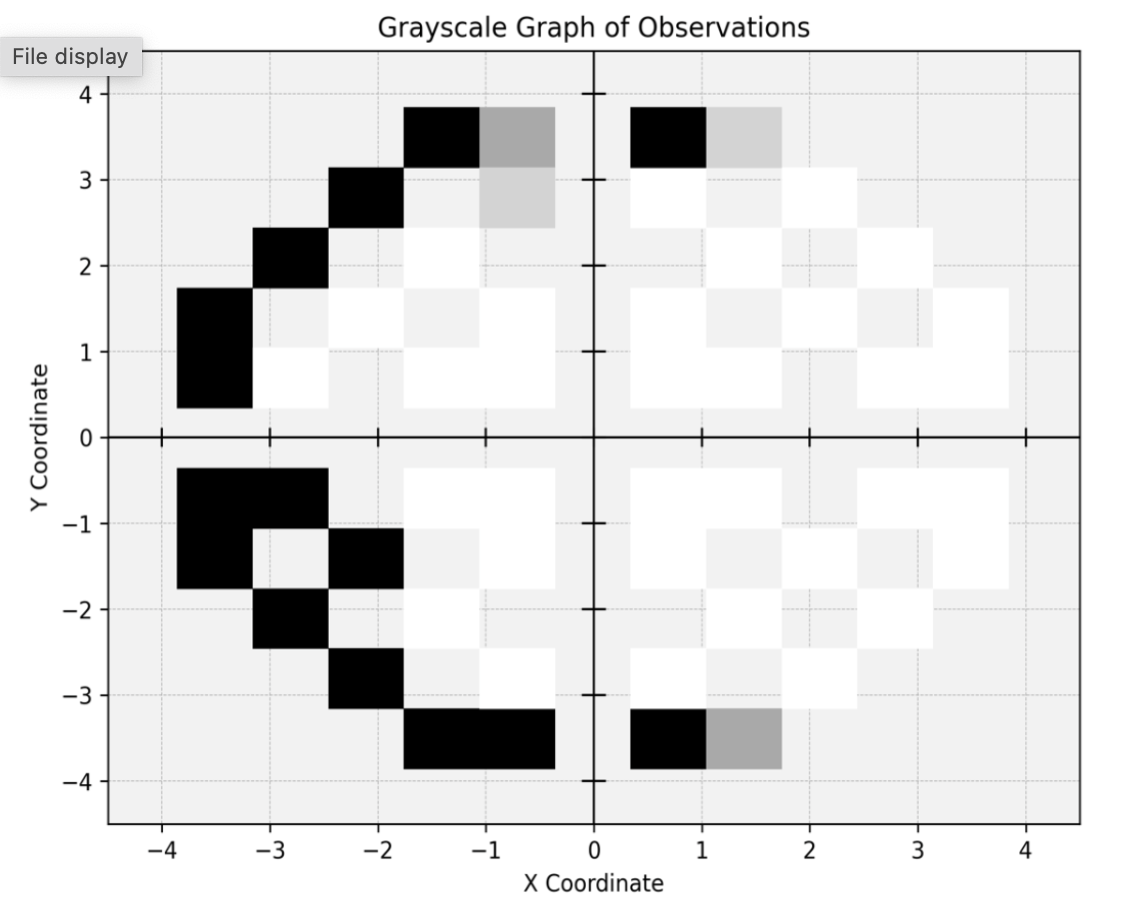
\includegraphics[width=\textwidth]{dissertation/images/participant2_gs_r.png}
        \caption{Gray scale}
        \label{fig:implemented_gs}
    \end{subfigure}
    \hfill
    \begin{subfigure}[b]{0.4\textwidth}
        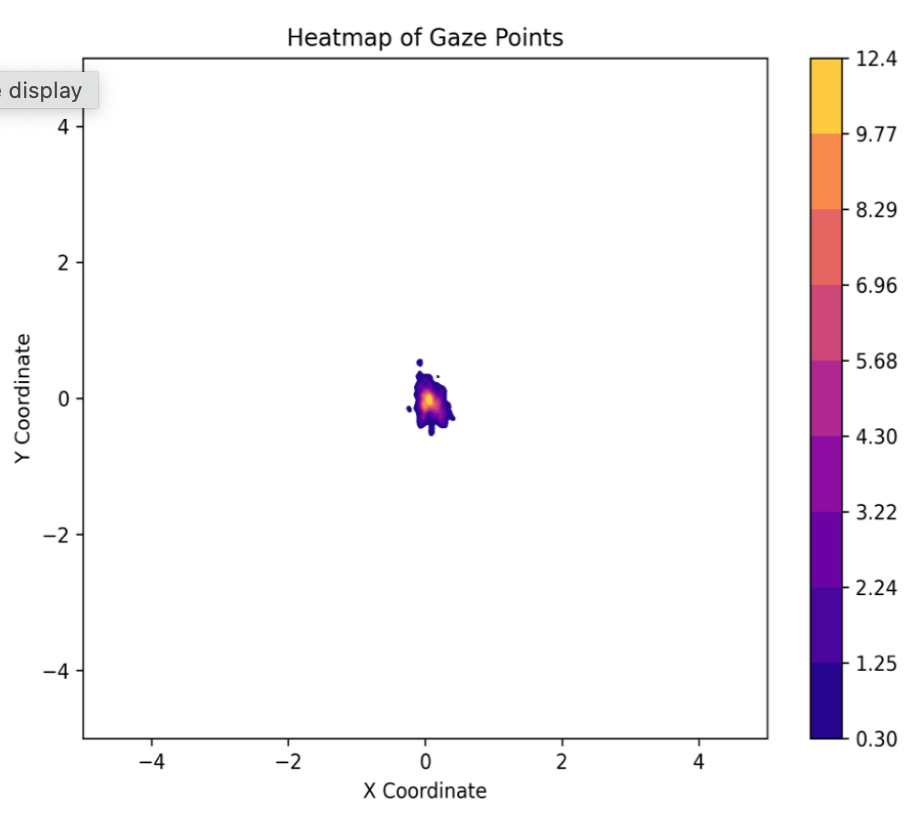
\includegraphics[width=\textwidth]{dissertation/images/participant2_hm_r.png}
        \caption{Heat Map}
        \label{fig:implemented_hm}
    \end{subfigure}
    \hfill
    \begin{subfigure}[b]{0.5\textwidth}
        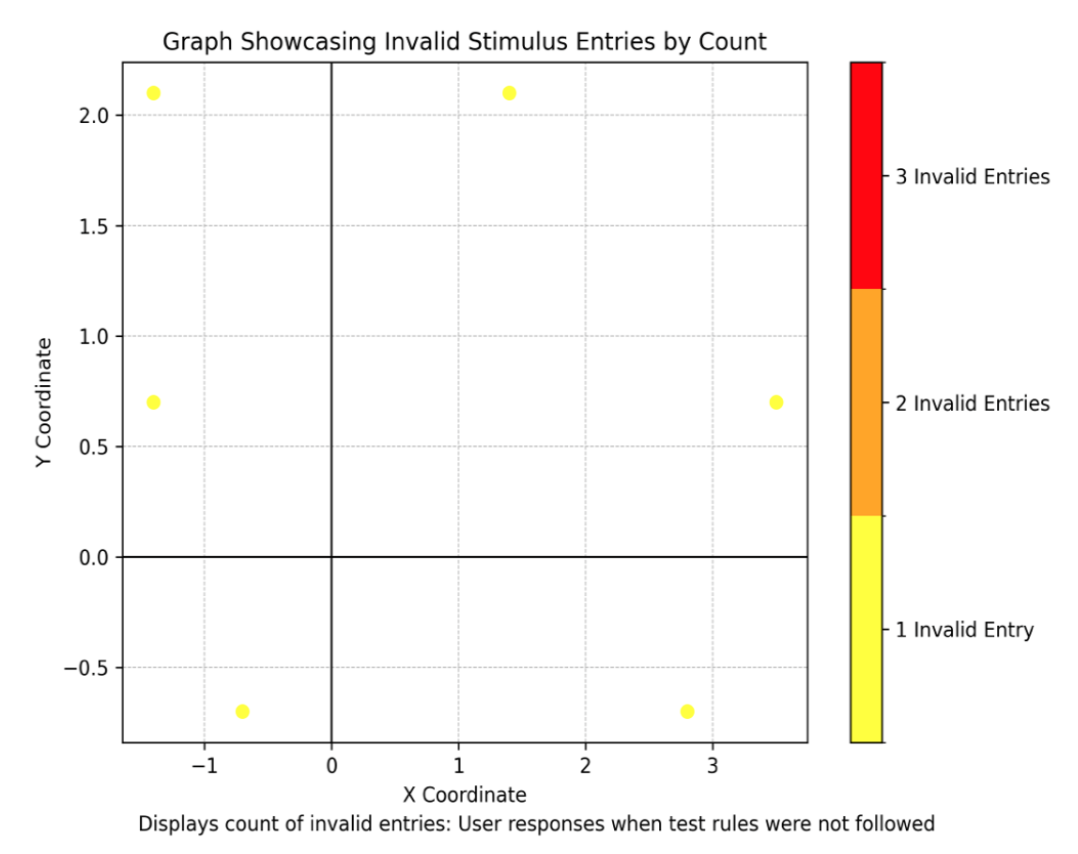
\includegraphics[width=\textwidth]{dissertation/images/participant2_iv_r.png}
        \caption{Invalid Points}
        \label{fig:implemented_iv}
    \end{subfigure}
    \caption{A showcase of three graphs generated by their respective scripts. These three graphs were from Participant 2 (right eye).}
    \label{fig:implemented_graphs}
\end{figure}
Our graphing scripts are called by ReportScripts.cs. This goes through each external python script and calls it before finally calling the PDF\_generate.py script. Although there shouldn't be any errors, our ReportsScripts.cs ensures all logging is redirected to our Unity console. All scripts take in a file path that points to the raw data. Finally, our PDF\_generate.py is called. This utilises the graphs and calculates a number of useful metrics for our report. Firstly, it uses test\_info.txt to generate information on our stimulus type, test time, response time and how user fixation information is collected. It also reads in our graphs stored in processed/. We use a package called reportlab to format and save our pdf to report/. To see a full report please refer to \ref{appendix:Sample_report}.
\section{Chapter Summary}
This chapter laid out our practical implementation of our research project covering our hardware, software and the Software Development Kits (SDKs) we used to enable our projects functional requirements and design. In hardware we delineated the specifications of our HMD, as well as the eye-tracking capabilities it came with. In Virtual Reality Environment we discussed Unity, the platform we used to develop our project. We discussed a number of SDKs that enabled us to use eye-tracking as well as enable interaction between the user and our environment. Next, we looked into the overall structure of our program - we divided our program into three parts, our Main menu, our testing environment with visual feedback and our testing environment with no visual feedback. We then moved onto how our testing algorithm worked in practise, and how it used helper functions to collect necessary information for the raw output of a test run. Finally, we talked about our python scripts to turn our raw data into graphs and metrics, and then into an auto-generated PDF detailing the users test results. In the next chapter we will evaluate our implementation by conducting a user evaluation in addition to a individual study with a user who has right-side homonymous hemianopia.
%==================================================================================================================================
\chapter{Evaluation} 
In this chapter, we outline our experimental procedure used to evaluate the visual field test in VR with the aim of answering our research question proposed in Chapter 1. We present the results of our user study and experiment and discuss how these answer our question and relate to wider literature.

\section{Guidance}
\begin{itemize}
    \item How good is your solution? How well did you solve the general problem, and what evidence do you have to support that?
    \item
        Ask specific questions that address the general problem.
    \item
        Answer them with precise evidence (graphs, numbers, statistical
        analysis, qualitative analysis).
    \item
        Be fair and be scientific.
    \item
        The key thing is to show that you know how to evaluate your work, not
        that your work is the most amazing product ever.
\end{itemize}


\section{User Evaluation}
Due to the intended use of this virtual reality system as a visual field testing program it was important to understand the usability of this system through a user evaluation. The primary objective of of this section is to identify any potential usability challenges with the current system as well as gather feedback on the overall user experience. Additionally, we can use the test results gathered from our users in this evaluation to compare and analyse our test conditions in Section \ref{evaluation:Visual_Feedback}. Our evaluation was conducted on eight undergraduate students with non having experience of a visual field test of any kind. Additionally we collected responses from an individual study with a participant with right-side homonymous hemianopia (Background: \ref{background:VFT_Hemianopia}, and Individual Study: \ref{individual_study}).
\subsection{Methodology}
Firstly, the user was given an introductory script to read-over (see \ref{appendix:introduction}). This contained an outlined version of the methodology as well as mandatory points from the School of Computing Science Ethics Checklist (see \ref{appendix:ethics}). After going over any questions they had, the user evaluation began.

Participants underwent testing in two parts, each corresponding to one eye. They would either participate in a test with visual feedback or one with no visual feedback. This test condition as well as which eye was tested first was dictated by a Latin square we produced (see \ref{appendix:latin_square}) to mitigate potential order effects. Once the user was seated we began by calibrating their eye using the HTC Vive's built-in eye-tracking calibration software. The user then put their eye patch on and was put into the main menu to familiarise themselves with the VR environment. Once they were ready they used their controller to navigate to the correct testing environment deepening on their test condition. Here the user was reminded to keep their focus on the central point during the entirety of the test. They were reminded of the meaning of the visual feedback if that was their test condition, red suggesting the user is not looking at the centre, green suggesting they are, and orange to represent that the test has finished or has not began. Once they were clear of the test procedure they could begin the test. All testing was done with the Standard\_Test.txt (see \ref{appendix:standard_test}) setup which should take approximately 6-7 minutes. 

After the first eye test had concluded the user was instructed to take off their headset. They were then give a short survey asking them about the comfort using the equipment's (see \ref{appendix:US_part_1_1}), if they had any symptoms of cybersickness and finally how focused they remained during the test. After a short optional break testing resumed, with the other eye.

The user put the eye patch on there second eye and began the test with the same test condition throughout. After the same procedure, they were given the same short survey. Finally the user was given a longer post-evaluation survey. This collected information on the value of instruction given, if maintaining their gaze on the central stimuli, if they thought the feedback was helpful, if the duration was reasonable as well as the opportunity to provide comments if they wished. Finally the user was debriefed, inline with the School of Computing Science. To see the full debrief reference \ref{appendix:debrief}.
\subsection{Limitations}
It is important to acknowledge potential limitations arising from this methodology. Firstly, by removing the HMD to put on the eye patch, the calibration of the eye-tracking was likely affected. Although eye-tracking was found to be fairly reliable the Vive documentation recommends eye-tracking be calibrated every time the HMD is adjusted. This means there is likely inconsistencies or incorrect data within the eye tracking output. Secondly, there is a possibility of a learning effect. While the Latin square design aimed to mitigate any ordering effect, we cannot definitively conclude an absence of a learning effect. It is also important to recognise that there is a likelihood that participant fatigue effects testing results. For participants to keep complete focus on the central stimulus over a two tests is unlikely. Hence the Latin square was also used to mitigate this affect. Finally, the number of participants in our study is relatively small. With only 8 participants, our test conditions will only have four participants each if we follow the Latin square (plus one participant in our individual user study). 
\section{Usability Results}
This section will focus on evaluating the usability of our system, inline with our aim of making a usable and comfortable testing system. Based off results from the survey we can collect some quantitative data to evaluate this. Additionally we can use comments from our participants we collected to gain insight. To see the responses in full from our user survey consult \ref{appendix:full_survey_results}.
\subsection{Cybersickness in VR}
Cybersickness, as we defined in our background (see \ref{background:VR}) is a broad term used to describe feelings of nausea, dizziness and light-headedness. It can be caused by the weight of the headset and a lack of synchronisation between the user and their actions. Furthermore the screens used by the HMD can cause a number of symptoms. We collected data about such symptoms from our participants after both phases of testing.

Below in tables \ref{table:eye_strain}, \ref{table:general_discomfort} qand \ref{table:drowsiness} we can see user responses across both test condition to the question, 'answer the following questions on symptoms. I felt:'. User responses to this question were taken after their first and second eye was tested. This included responses from eight participants from our user study and our individual case study (see \ref{individual_study}).

Eye strain was prevalent amongst participants, we can see in Figure \ref{table:eye_strain} that 88.9\% of users reported some variation of eye strain after the first phase of testing. The distribution of eye strain is made up of 55.5\% in the 'A little' category followed by 11.1\% in 'Not at all,' 'Somewhat,' 'Often,' and 'Throughout'. However, the overall frequency of eye strain after Phase 2 decreases to 66.6\%, with 33.3\% experiencing no symptoms at all. There was a higher concentration of users experiencing more significant symptoms. The change in symptom perception suggests a habituation to the virtual reality environment; however, those with more pronounced symptoms may have experienced a more noticeable experience of symptoms.
\begin{table}[h] 
    \centering
    \caption{Comparison of Eye Strain Frequency across both testing phases}
    \begin{tabular}{|c|c|c|c|c|c|}
        \hline
        \textbf{Eye-Strain Frequency} & Not at all & A little & Somewhat & Often & Throughout \\
        \hline
        Phase 1 (First Eye) & 11.1\%  & 55.6\% & 11.1\% & 11.1\% & 11.1\%\\
        \hline
        Phase 2 (Second Eye) & 33.3\% & 11.1\% & 22.2\% & 22.2\% & 11.1\%\\
        \hline
    \end{tabular}
    \label{table:eye_strain}
\end{table}

When we tabulate our users responses on the same question regarding General discomfort (\ref{table:general_discomfort}) and Drowsiness (\ref{table:drowsiness}), we see further evidence supporting our theory of habituation to the virtual reality environment. The data suggests a trend towards a lower frequency of both symptoms in Phase 2 compared to Phase 1. 
In Phase 1 a significant portion of participants experienced some level of general discomfort (55.6\%) and drowsiness (44.4\%) compared to a far smaller percentage in Phase 2 with general discomfort (44.4\%) and drowsiness (22.2\%). Furthermore, there is once again appears to be a decrease in symptom severity, other than one exception with one participant increasing their drowsiness frequency to 'Somewhat'
\begin{table}[h]
    \centering
    \caption{Comparison of General Discomfort Frequency across both testing phases}
    \label{table:general_discomfort}
    \begin{tabular}{|c|c|c|c|c|c|}
        \hline
        \textbf{General Discomfort Frequency} & Not at all & A little & Somewhat & Often & Throughout \\
        \hline
        Phase 1 (First Eye) & 44.4\%  & - & 44.4\% & 11.1\% & - \\
        \hline
        Phase 2 (Second Eye) & 55.6\% & 22.2\% & 22.2\% & - & - \\
        \hline
    \end{tabular}
\end{table}

\begin{table}[h]
    \centering
    \caption{Comparison of Drowsiness Frequency across both testing phases}
    \label{table:drowsiness}
    \begin{tabular}{|c|c|c|c|c|c|}
        \hline
        \textbf{Drowsiness Frequency} & Not at all & A little & Somewhat & Often & Throughout \\
        \hline
        Phase 1 (First Eye) & 55.6\%  & 44.4\% & - & - & -\\
        \hline
        Phase 2 (Second Eye) & 77.8\% & 11.1\% & 11.1\% & - & -\\
        \hline
    \end{tabular}
\end{table}

Symptoms such as sweating, apathy and  headaches were all recorded by no more than two participants each in both phases. Furthermore, nausea was recorded in Phase 2 as 'often' by one participant. The results appear so show symptoms of cybersickness were prevalent throughout testing, especially eye strain and general discomfort. However, due to our small sample size we cannot definitively conclude that the prevalence of these symptoms are accurately represented in our findings. To see the full results graph of symptoms from our participants please consult \ref{fig:symptoms}.
\newpage
\subsection{Test Equipment Comfort}
In this section we will discuss the comfortability of the headset based off the results collected in our user evaluation. We aim to understand user comfort as it contributes to overall usability of our project and is especially important as user discomfort could lead to distraction amongst our participants during testing. Using Figure \ref{fig:comfort_1} and \ref{fig:comfort_2} we compare reported comfort of both our HMD and eye patch during testing.
\begin{figure}[htbp]
    \centering
    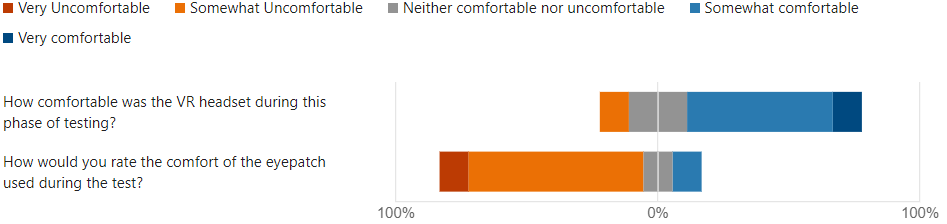
\includegraphics[width=0.9\linewidth]{dissertation/images/Comfort_Part_1.png}    
    \caption{Equipment comfort evaluation for Phase 1} \label{fig:comfort_1}
    
    \vspace{1cm}
    
    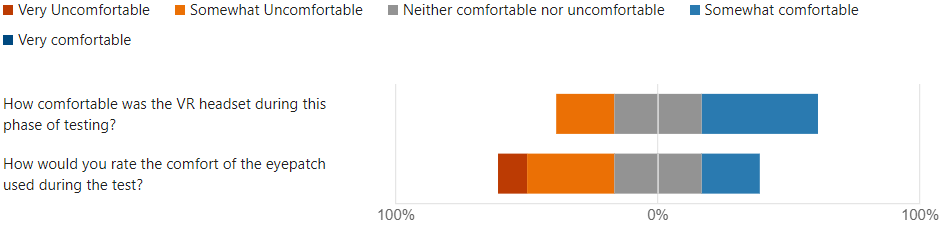
\includegraphics[width=0.9\linewidth]{dissertation/images/Comfort_Part_2.png}    
    \caption{Equipment comfort evaluation for Phase 2} \label{fig:comfort_2}
\end{figure}
\newline
\textbf{VR Headset Comfort}: In phase 1 the majority of participants rated the VR headset as 'somewhat comfortable' (55.6\%) followed by 'neither comfortable nor uncomfortable' (22.2\%). Only a small percentage of participants found the VR 'somewhat uncomfortable' at (11.1\%) and 'very comfortable' (11.1\%). in Phase 2 we see the distribution shift, with a higher percentage of participants rating it 'neither comfortable nor uncomfortable' and 'somewhat uncomfortable'. 

\textbf{Eye Patch Comfort}: The eye patch was initially rated less favourably than the headset with 77.8\% of participants finding it uncomfortable in some capacity. The distribution shifts slightly in the second Phase with 44.4\% of users finding it uncomfortable in some capacity, however it is never rated 'very comfortable' and only 2 participants rate it as comfortable in some capacity. 

We can definitively conclude that users generally find the HMD more comfortable than our eye patch. However, as both work in conjunction during testing it is important to discuss limitations with this approach based off our data. Firstly, it is clear that the eye patch approach to testing is neither comfortable, and thus it does not create a usable system. This could have exacerbated many of the symptoms discussed in our previous section. Furthermore, discomfort likely introduces  a confounding variable into our user test results as their responses could be influenced by discomfort. This gives us a potential for further work, as we could look into alternative solutions for our eye patch.


\subsection{Testing Duration}
In this section we will discuss the duration of our test. Firstly, the mean test time was 454.925 seconds, with a lower bound of 362.91 seconds and an upper bound of 731.96 seconds. This is inline with current HVF analysers which have test times of \( \sim300-600 \). 

When users were asked if the duration of the test was reasonable, 89.9\% of participants answered yes with 11.1\% answering no. This implies that the testing length was likely a reasonable duration for most participants. However, a few comments appeared to suggest otherwise despite the high number of 'yes' responses. Comments such as 'at the least minute the eye strain was a little too much. 5 minutes [of testing] at most?', 'slightly too long. could do a shorter test?' and 'reasonable, but I would have preferred it to be faster as it started to get slightly uncomfortable' suggests although participants may have found the test reasonable there is a strong demand for slightly shorter test times, perhaps around the 5 minute mark, or in our case, around the lower bound of our test time.

Furthermore, it would be beneficial to understand the habituation affect that may be present during testing. We hypothesise, as the test continues users may perform better as they begin to understand the process and shape of the stimuli, before eventually dropping off as their concentration diminishes. It would be worth exploring the relationship between test duration and performance.

\subsection{Overall Usability Findings}
We conclude that our system is currently usable, but that there are a number of alterations that could be made to increase its usability. We come to this conclusion firstly, based off our previous evaluations but also, due simply to our users response to the question: 'How would you rate your overall experience with the automated visual field test in VR?'. Table\ref{table:overall_experience} shows a positive response from users, with no ratings going below 'Good'. To summarise, although our findings suggest the eye-patch was uncomfortable for many users, it did not make the system unusable. Continuing, it appears a number of users acclimatised to the eye-patch, while some users began to find the virtual reality headset less comfortable in the second Phase of testing, as shown by the shift in distribution between Figure \ref{fig:comfort_1} and Figure \ref{fig:comfort_2}. Furthermore, the data suggests that the majority of participants had symptoms of eye strain and general discomfort in the first phase, but this subsided in the second phase as they habituated to the virtual environment - apart from a small number of participants who felt symptoms intensify. General discomfort subsides in the second phase with both the number of users experiencing symptoms lessening and its distribution shifting towards 'Not at all'. A similar pattern occurs with Drowsiness with the exception of one participants symptom increased their frequency to 'Somewhat'.
\begin{table}[h]
    \centering
    \caption{How would the user rate their overall experience with visual field testing in VR}
    \label{table:overall_experience}
    \begin{tabular}{|c|c|c|c|c|c|}
        \hline
        \textbf{Rating} & Very Poor & Poor & Average & Good & Very Good \\
        \hline
        User Responses & - & - & - & 89\% & 11\%\\
        \hline
    \end{tabular}
\end{table}

With our findings summarised, we come back to our conclusion, that our system is currently usable when performing its functionality however there are a number of improvements to be made. Firstly we hypothesis by removing the eye-patch and monocular streaming to the HMD, we could potentially remove the requirement of the eye-patch. This would likely increase comfortability and usability as a whole. Secondly, it would be beneficial to provide tests of different lengths, for instance, tests at the 200,300 and 500 second mark. Longer tests could be used for patients with specific conditions such as glaucoma and hemianopia to track progression or regression of the condition. Finally - as mentioned previously - it would be beneficial to understand the habituation effects that may be present. A user who conducts more tests may have better results as they understand what to expect in terms of stimulus size, location and also the methodology of the test.

\section{Impact of Visual Feedback on Test Results} \label{evaluation:Visual_Feedback}
We hypothesised that visual feedback during user testing would improve the validity. We therefore put forward:
\begin{itemize}
    \item \textbf{Null Hypothesis (H0)}: There is no significant difference in the mean percentage of valid responses between the condition with visual feedback and the condition without visual feedback
    \item \textbf{Alternative Hypothesis (H1)}: The mean percentage of valid responses is significantly higher in the condition with visual feedback compared to the condition without visual feedback.
\end{itemize}
With these, and we can conduct a t-test to determine if there is a statistically significant difference in the mean percentage of valid responses between the two conditions. 
\begin{figure}[htbp]
    \centering
    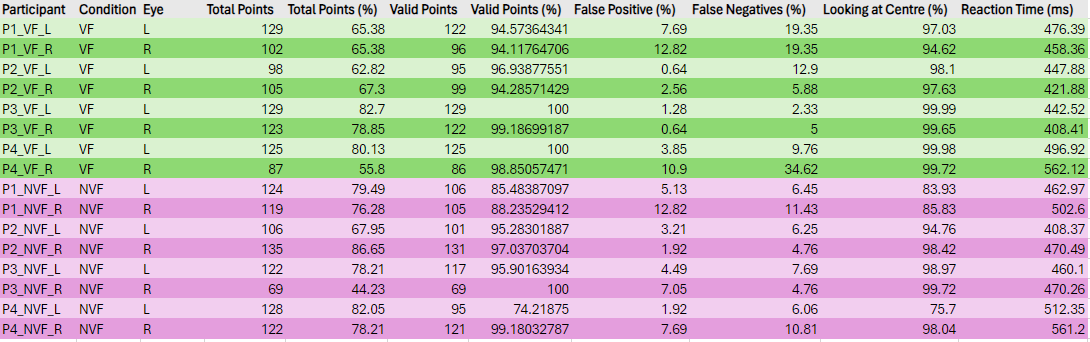
\includegraphics[width=1\linewidth]{dissertation/images/Results.png}    

    \caption{A table of results. Includes metrics from P1-P8. Excluding Individual Study.}
    \label{fig:results} 
\end{figure}
\newline
We can use results from Figure \ref{fig:results} to calculate mean ($\mu$) and standard deviation ($\sigma$) to compute our t-test value. \newline
\newline
$Mean_{VF}: 98.21034273 \newline 
Mean_{NVF}: 91.91749228 \newline
\newline
Standard Deviation_{VF}: 2.599364617 \newline
Standard Deviation_{NVF}: 8.780507569 
$

Given the results from these calculations we conclude that our \textbf{t-test equals: 1.943705608}. As degrees of freedom (df) is equal to:
$df = n_1 + n_2 -2$
we can use our degrees of freedom (df=6), our one-tailed t-test ($\alpha$) and our significance level (0.05) to consult a T-Distribution table of critical values\footnote{https://statisticsbyjim.com/hypothesis-testing/t-distribution-table/} to find the critical value.

Given the critical value is: 1.943, and our t-value was: 1.944 (3 s.f.) we can reject the null hypothesis and conclude that there is a statistically significant difference in the mean percentage of valid response between the condition with visual feedback and the condition without visual feedback at the 0.05 significance level. Specifically, the mean percentage of valid responses in the condition with visual feedback is statistically significantly  greater than the mean percentage in the condition without visual feedback.

However, it is important to understand the limitations that are present in this study. Firstly, the sample size is relatively small with only 8 participants or 16 tests being conducted (one test per eye). A larger sample size would provide greater statistical power, and would likely enhance the robustness of our study. Furthermore, all eight participants were of similar age and background (19-22, undergraduate students respectively with no eye conditions) and as such this studies findings may not be Representative of the wider population, specifically for users with neuro-ophthalmological conditions such as our participant from our individual study.





[SUMMARY BELOW]
With the results of our t-test supporting our alternative hypothesis, indicating that visual feedback during user testing leads to a statistically significant increase in the mean percentage of valid responses compared to testing without visual feedback, we suggest that incorporating real-time feedback into test procedure can enhance the validity of testing results. 
Make sure you present your evidence well. Use appropriate visualisations, reporting techniques and statistical analysis, as appropriate.

\section{Individual Case Study} \label{individual_study}
If you visualise, follow the basic rules, as illustrated in Figure 
\begin{itemize}
\item Label everything correctly (axis, title, units).
\item Caption thoroughly.
\item Reference in text.
\item \textbf{Include appropriate display of uncertainty (e.g. error bars, Box plot)}
\item Minimise clutter.
\end{itemize}

See the file \texttt{guide\_to\_visualising.pdf} for further information and guidance.



%==================================================================================================================================
\chapter{Conclusion and Further Work}    
Summarise the whole project for a lazy reader who didn't read the rest (e.g. a prize-awarding committee).
\section{Guidance}
\begin{itemize}
    \item
        Summarise briefly and fairly.
    \item
        You should be addressing the general problem you introduced in the
        Introduction.        
    \item
        Include summary of concrete results (``the new compiler ran 2x
        faster'')
    \item
        Indicate what future work could be done, but remember: \textbf{you
        won't get credit for things you haven't done}.
\end{itemize}
\section{Summary}
\section{Future Work}
\subsection{Quicker Testing Algorithm}
Testing times in the project were found to be overly long by participants in the user evaluation. [IS THIS TRUE?] Therefore, there is potential future work in improving the speed of testing by refactoring the testing algorithm. HVF analyser algorithms such as SITA from the background could significantly reduce testing times. The algorithm could dynamically change the response time and random interval inbetween each stimulus depending on the user - or even remove stimuli if the program is confident the users visual field has no imperfections in that area.

\subsection{Threshold Testing}
One primary element of HVF analyser testing that was not included in this project was threshold testing. As mentioned in the background, threshold testing refers to testing the level of light of a displayed stimulus that the user can see consistently. The light of the stimulus, measured logarithmically in decibels, would require a refactored testing algorithm as well as a function to handle translations between the logarithmic scale and Unity's linear scale. However by implementing threshold testing this could provide benefit by allowing operators to gauge the functional integrity of a patients retina and visual pathway.

\subsection{Industry-Norm Tests}
Furthermore, testing could follow industry conventions. Tests could adhere to standard conventions outlined in the background. This includes using tests such as the 24-2 and 10-2. These tests focus on different parts of the users visual field and thus enable the correct type of testing depending on the users condition. These tests would also save time as only the visual field that needs tested is tested. \citet{RuiaTripathy2021HVF} contains more information on conventional HVF testing formats.
\subsection{Mean-Deviation Visualisations}
Incorporating mean-deviation visualisations into the VR visual field report could offer insight into the users visual field data. Plotting mean deviations from age-matched norms would allow operators to identify regions of potential visual field loss or abnormalities. Datasets are sparse due to their medical nature however there is a publicly available set of HVF results by \cite{montesano2022uwhvf} on GitHub\footnote{https://github.com/uw-biomedical-ml/uwhvf}. Mean-Deviation could be calculated by age or using a custom metric such as threshold level. There are many comparison possibilities using this dataset, but importantly implementing mean deviation would adhere to current HVF test reports.


%==================================================================================================================================
%
% 
%==================================================================================================================================
%  APPENDICES  

\begin{appendices}

\chapter{Appendices}

Typical inclusions in the appendices are:

\begin{itemize}
\item
  Copies of ethics approvals (required if obtained)
\item
  Copies of questionnaires etc. used to gather data from subjects.
\item
  Extensive tables or figures that are too bulky to fit in the main body of
  the report, particularly ones that are repetitive and summarised in the body.

\item Outline of the source code (e.g. directory structure), or other architecture documentation like class diagrams.

\item User manuals, and any guides to starting/running the software.

\end{itemize}

\textbf{Don't include your source code in the appendices}. It will be
submitted separately.

\section{Implementation}
\subsection{Project Source Files} \label{appendix:source_files}
All files have been uploaded to the L4-Project University of Glasgow Moodle, in accordance with the requirements of this course. Furthermore it can be found at this GitHub Repository: https://github.com/AlfieMacintosh/L4-Project
\newpage
\subsection{Sample Test Report} \label{appendix:Sample_report}
\begin{figure}[htbp]
    \centering
    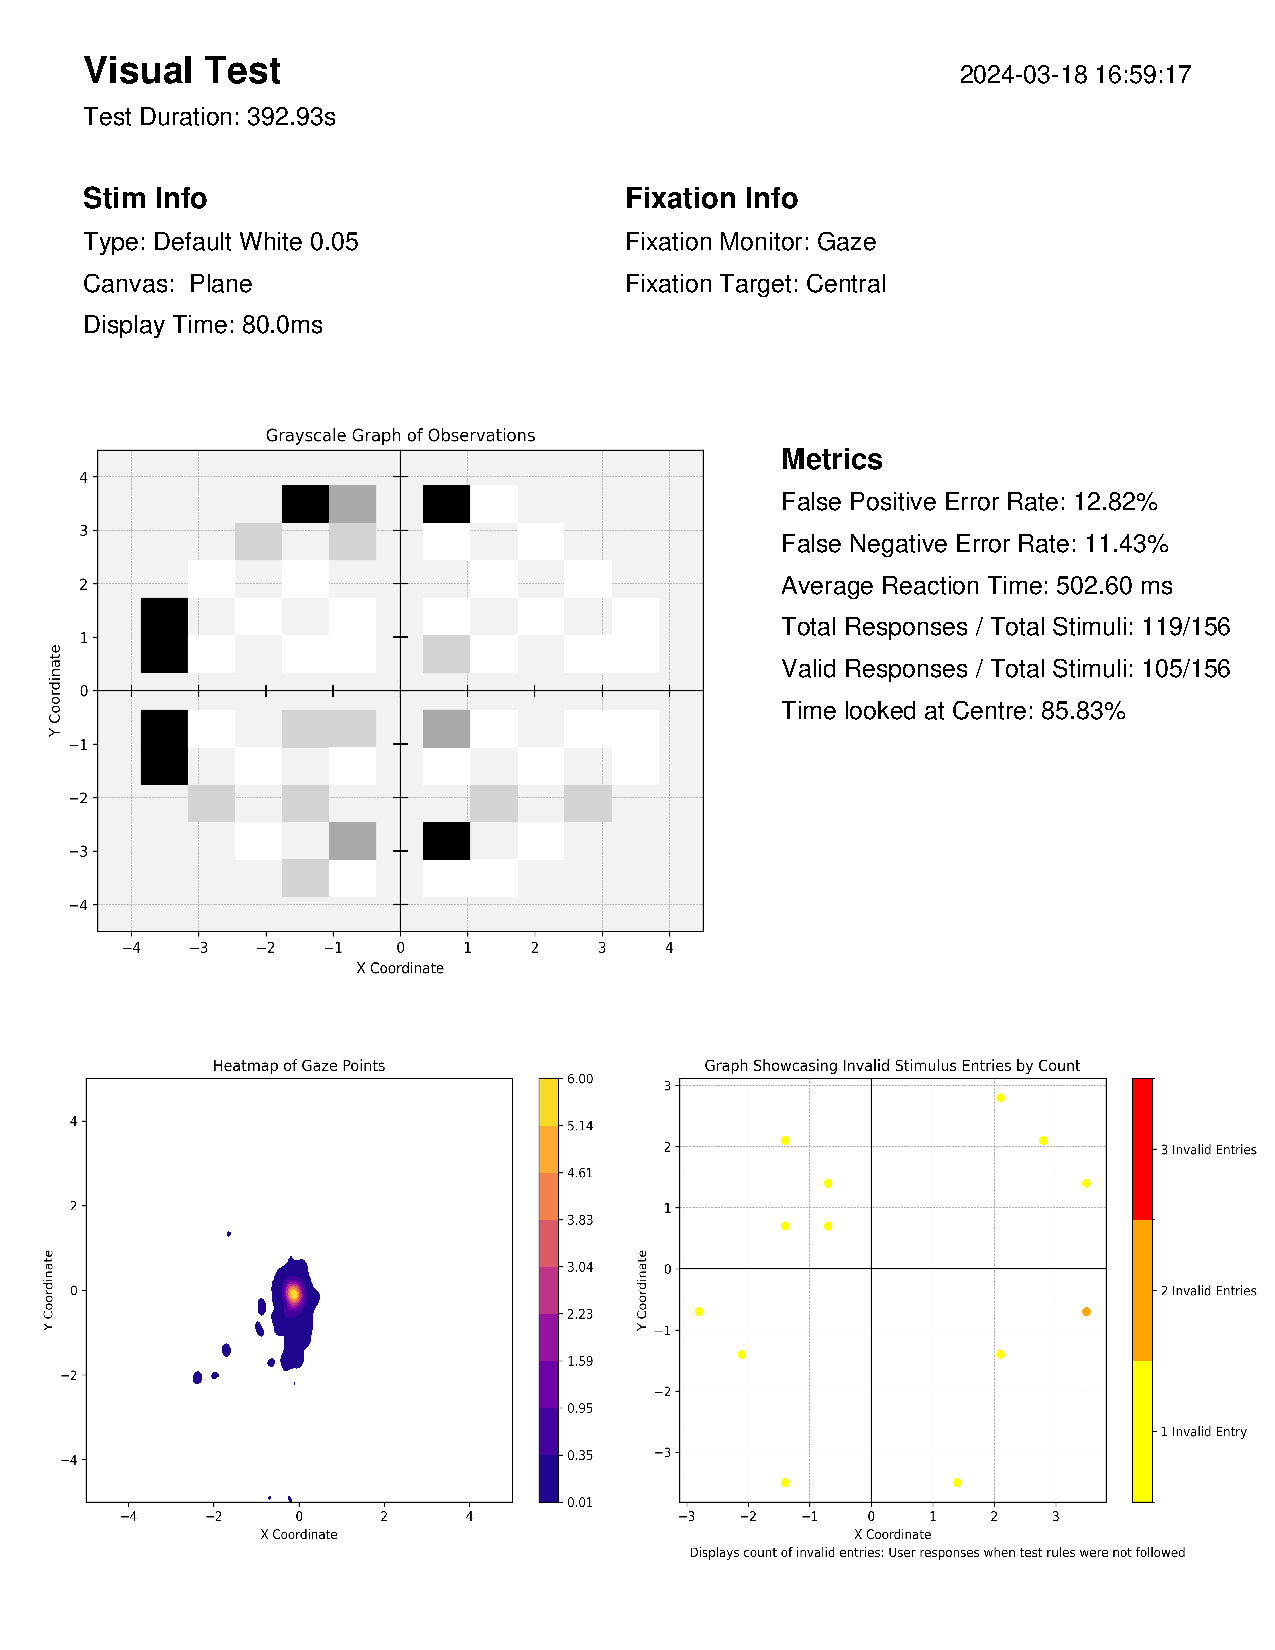
\includegraphics[width=0.8\linewidth]{dissertation/images/test_results.pdf}    

    \caption{A test report from Participant 5 (right eye). Showcasing the graphs from our reporting scripts as well as testing metrics.}
\end{figure}
\newpage
\section{Evaluation}
\subsection{Introduction} \label{appendix:introduction}
\begin{figure}[htbp]
    \centering
    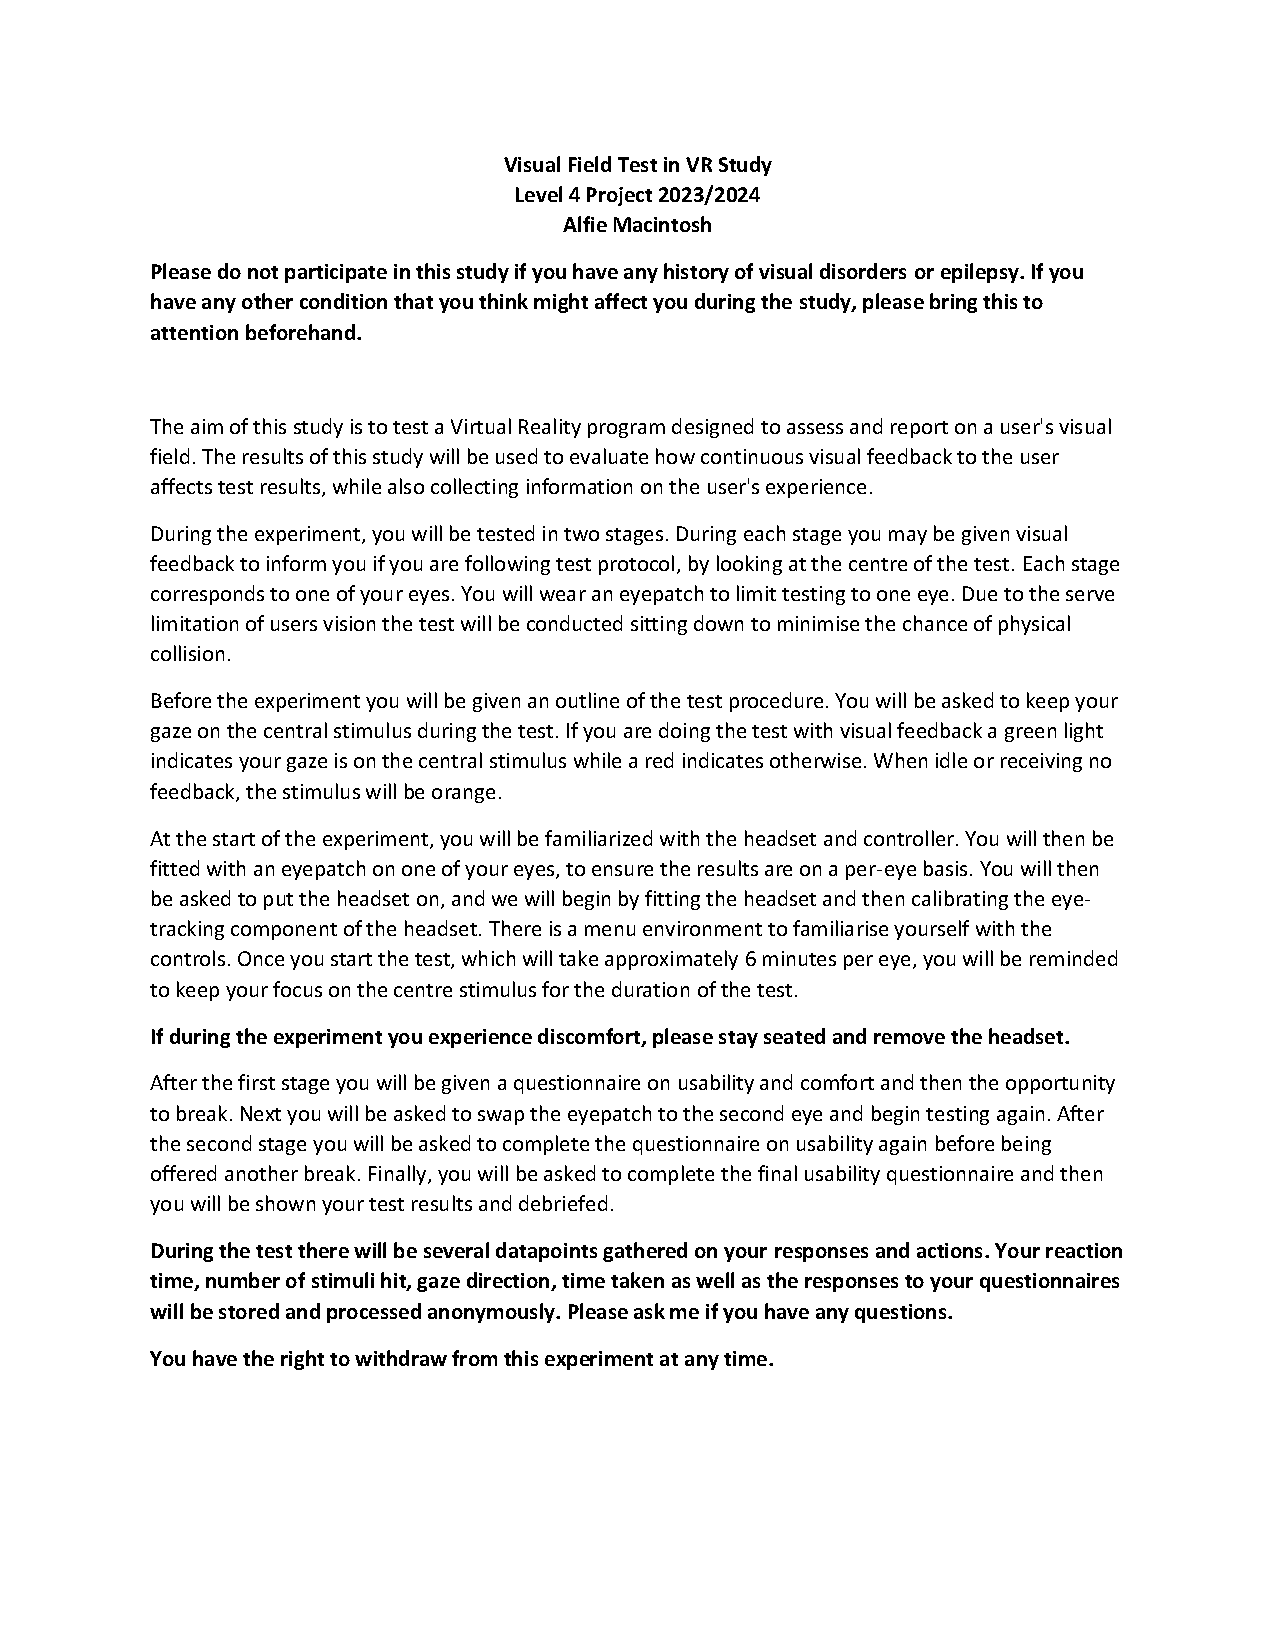
\includegraphics[width=0.9\linewidth]{dissertation/images/Introduction.pdf}    
    \caption{Introductory brief for users participating in study.}
\end{figure}
\newpage
\subsection{Debrief} \label{appendix:debrief}
\begin{figure}[htbp]
    \centering
    
\includegraphics[width=0.9\linewidth]{dissertation/images/Debrief.pdf}    
    \caption{Debrief for users participating in study.}
\end{figure}
\newpage
\subsection{Ethics Form} \label{appendix:ethics}
\begin{figure}[htbp]
    \centering
    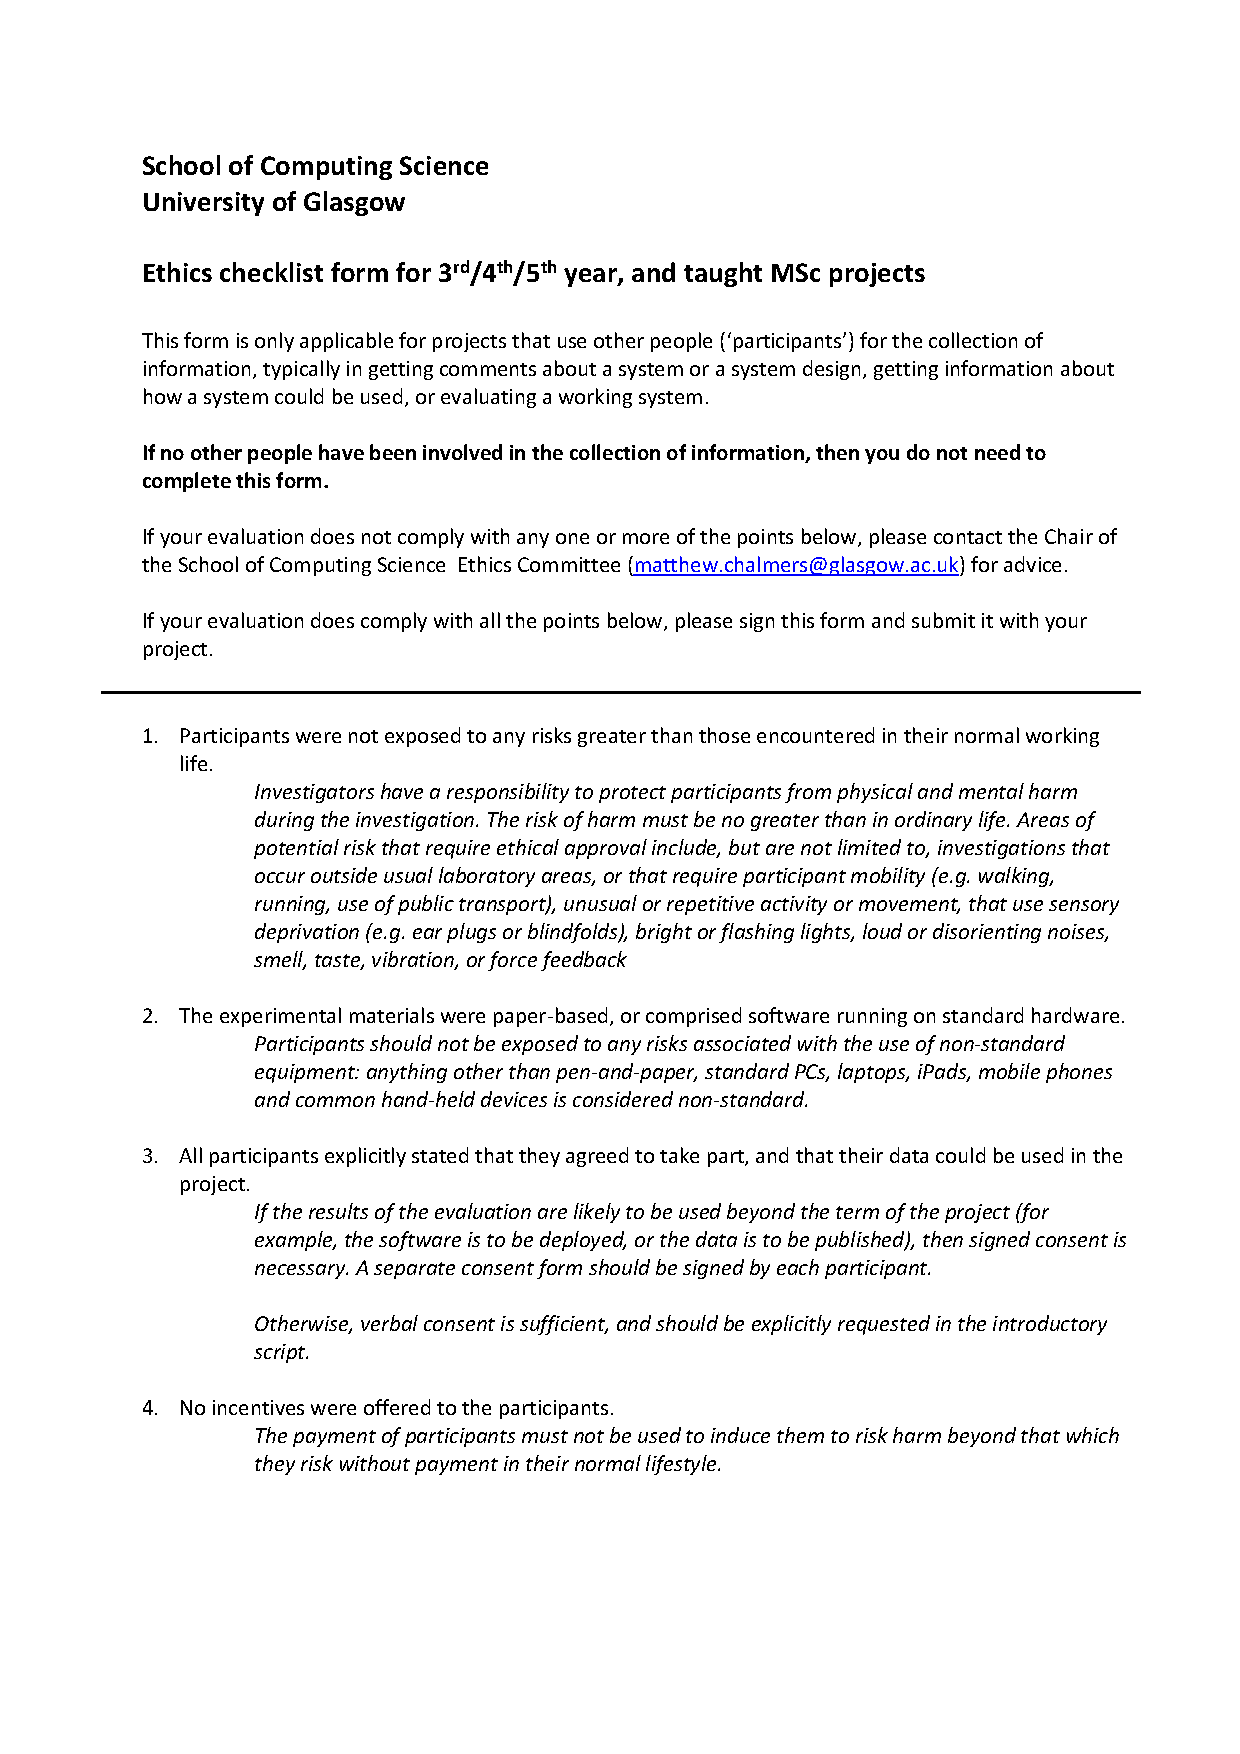
\includegraphics[page=1,width=0.8\linewidth]{dissertation/images/Ethics.pdf}   
    \caption{Filled out ethics form, inline with School of Computing Science Guidelines. Page 1/2.}
\end{figure}
\newpage
\begin{figure}[htbp]
    \centering
    \includegraphics[page=2,width=0.8\linewidth]{dissertation/images/Ethics.pdf}   
    \caption{Filled out ethics form, inline with School of Computing Science Guidelines. Page 2/2}
\end{figure}
\newpage
\subsection{Latin Square} \label{appendix:latin_square}
\begin{figure}[htbp]
    \centering
    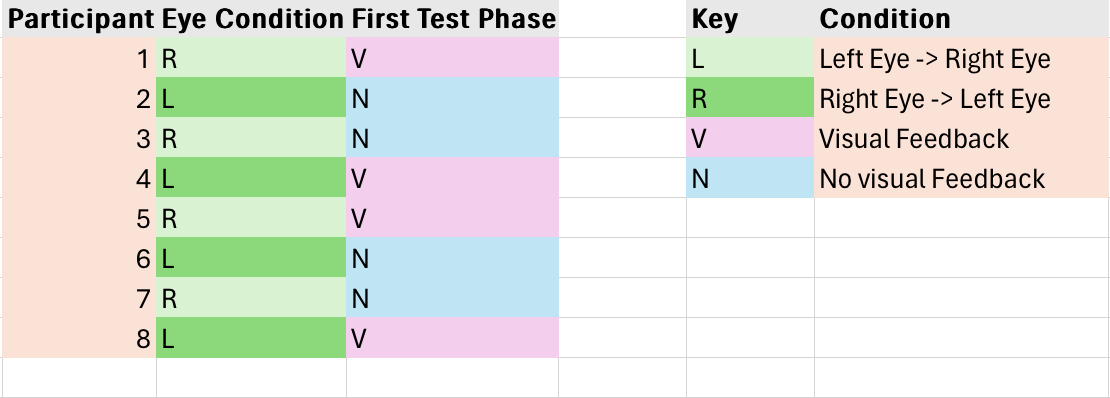
\includegraphics[width=0.9\linewidth]{dissertation/images/Latin Square.png}   
    \caption{Latin Square used to assign participants test conditions.}
\end{figure}
\newpage
\subsection{Inter-Study Usability Survey} \label{appendix:US_part_1_1}
\begin{figure}[htbp]
    \centering
    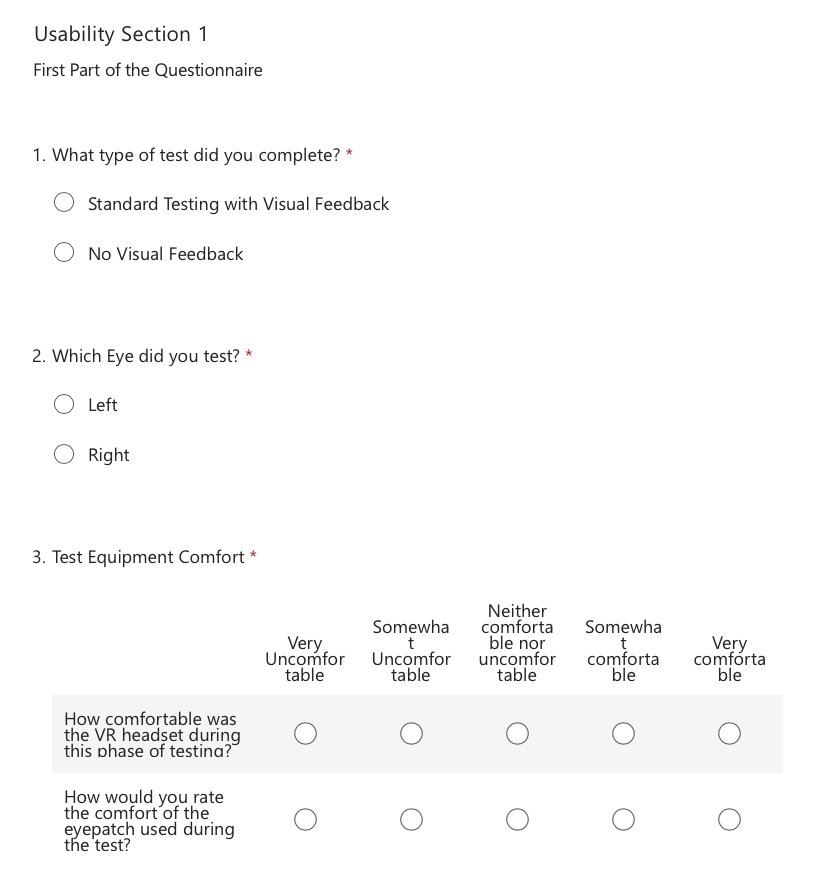
\includegraphics[width=0.9\linewidth]{dissertation/images/US_Part1_1.png}   
    \caption{Part 1/2 of the Usability Survey}
\end{figure}
\begin{figure}[htbp]
    \centering
    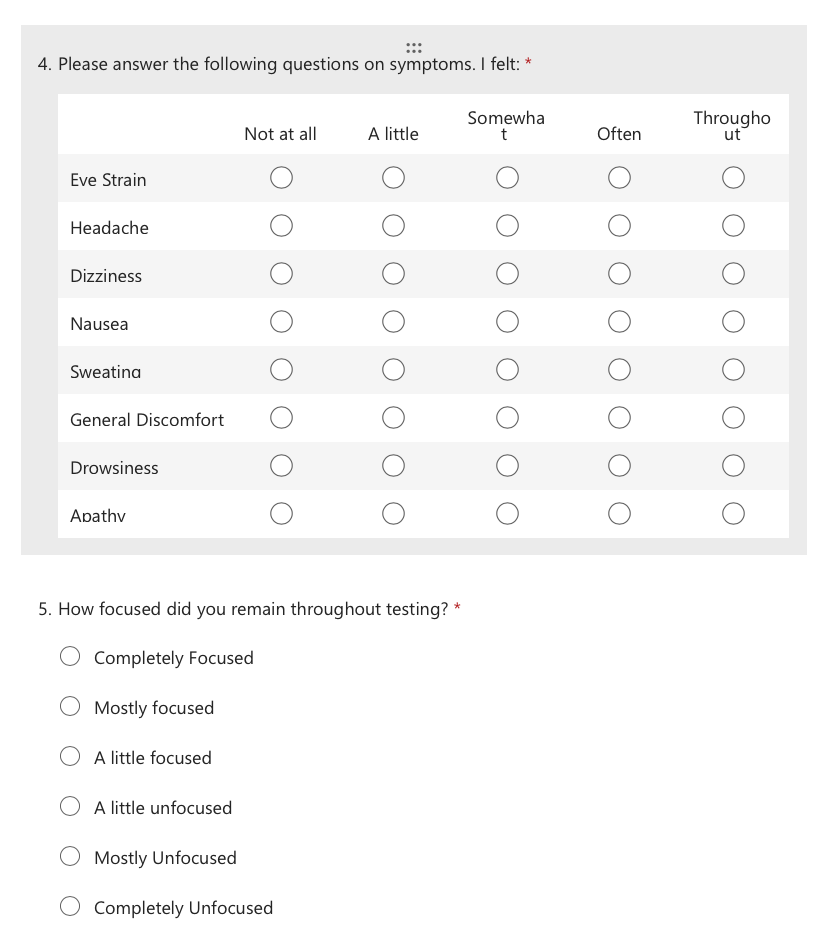
\includegraphics[width=0.9\linewidth]{dissertation/images/US_Part1_2.png}   
    \caption{Part 2/2 of the Usability Survey}
\end{figure}
\newpage
\subsection{Post-Study Usability Survey} \label{appendix:US_part_3}
\begin{figure}[htbp]
    \centering
    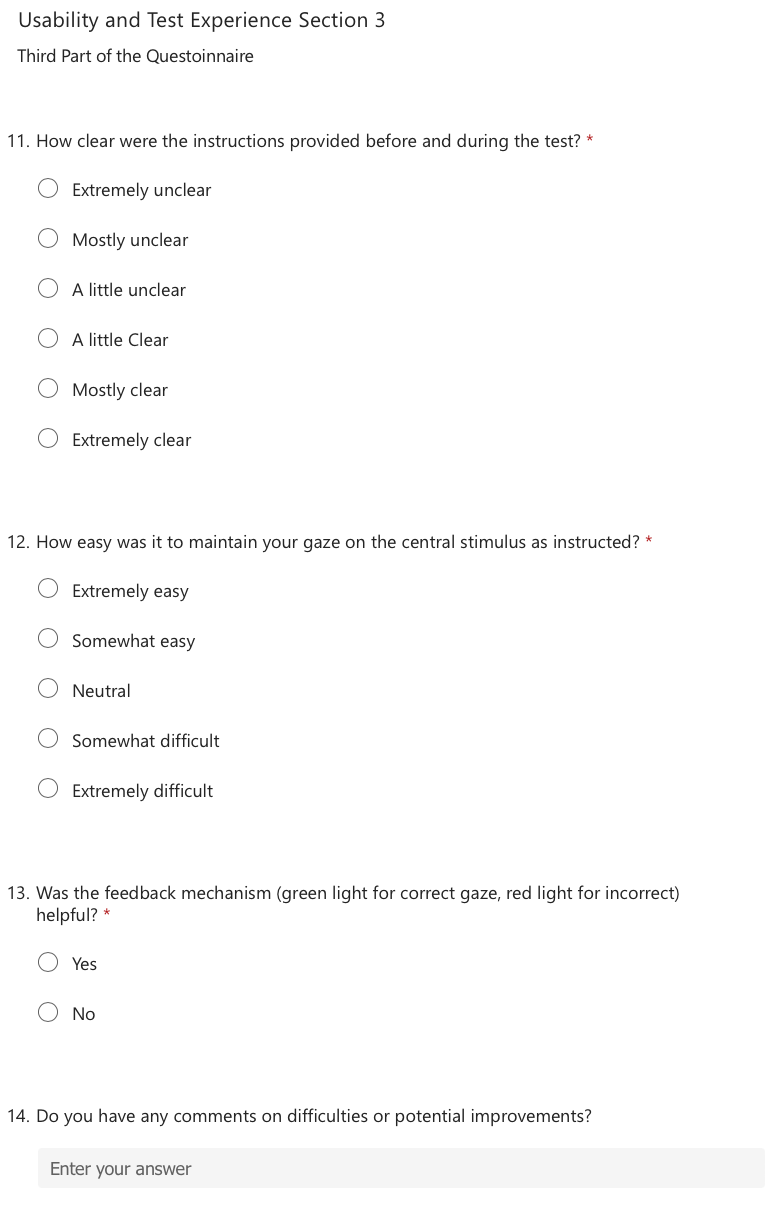
\includegraphics[width=0.7\linewidth]{dissertation/images/US_Part3_1.png}   
    \caption{Part 1/2 of the Post-Study Usability Survey}
\end{figure}
\begin{figure}[htbp]
    \centering
    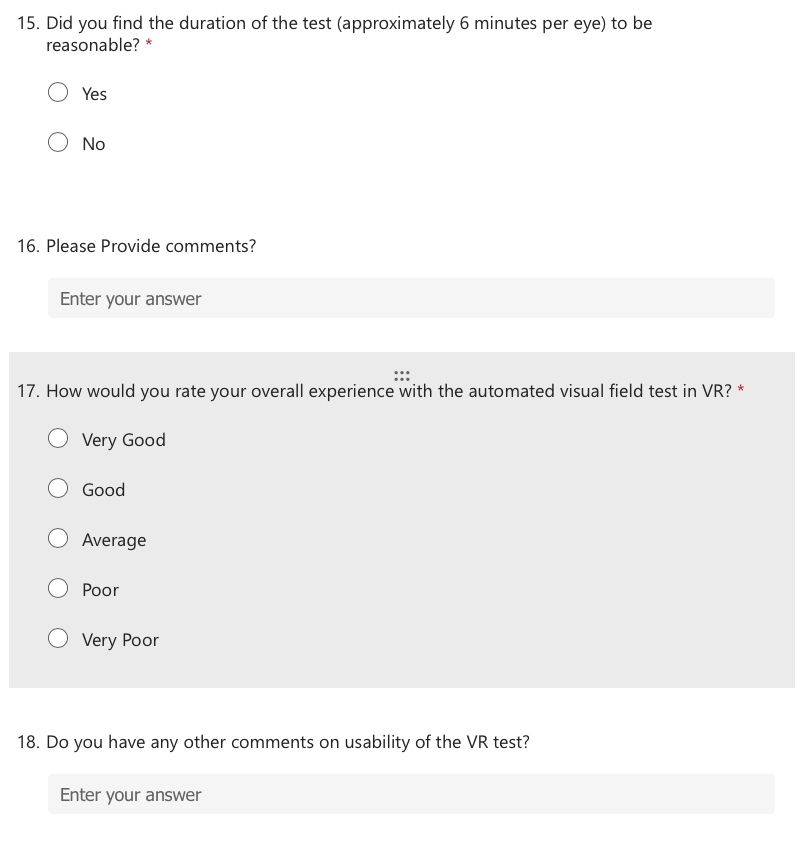
\includegraphics[width=0.9\linewidth]{dissertation/images/US_Part3_2.png}   
    \caption{Part 2/2 of the Post-Study Usability Survey}
\end{figure}
\newpage
\subsection{Standard Test Input} \label{appendix:standard_test}
\begin{figure}[htbp]
    \centering
    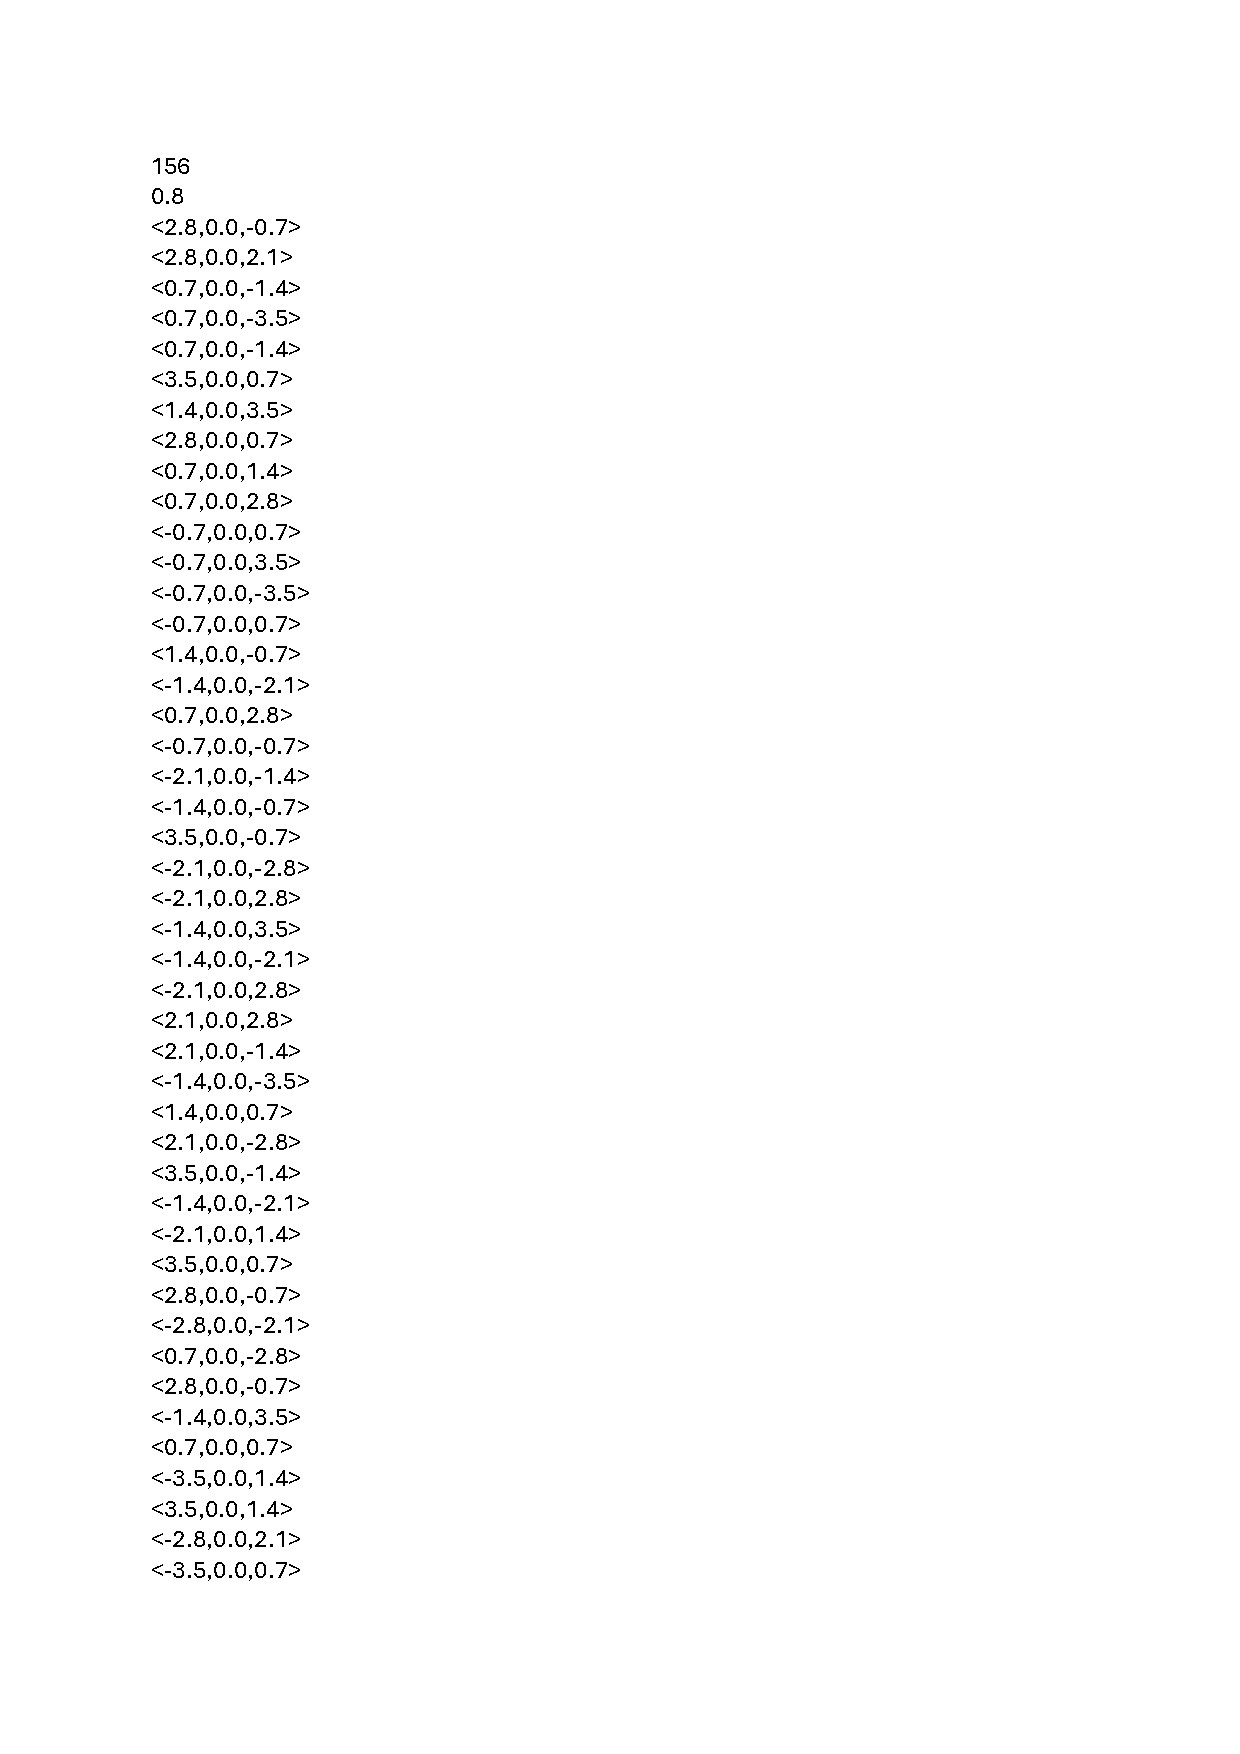
\includegraphics[page=1,width=0.8\linewidth]{dissertation/images/Standard_Test.pdf}   
    \caption{Exert from Standard Test Input. First line represents number of stimuli, second line is the response time,  the rest represent the local coordinates of the stimuli to be shown (relative to the canvas).}
\end{figure}
\subsection{User Symptoms} \label{fig:symptoms}
\begin{figure}[htbp]
    \centering
    \begin{subfigure}{0.95\textwidth}
        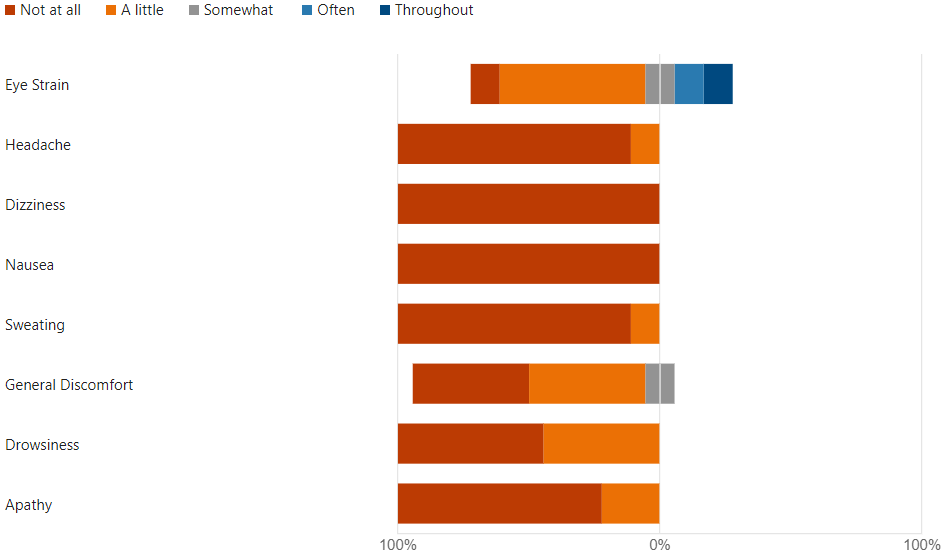
\includegraphics[width=\textwidth]{dissertation/images/Symptoms_Part_1.png}
        \caption{Responses after the users first eye was tested.}
        \label{fig:symptoms_part_1}
    \end{subfigure}
    \hfill
    \begin{subfigure}{0.95\textwidth}
        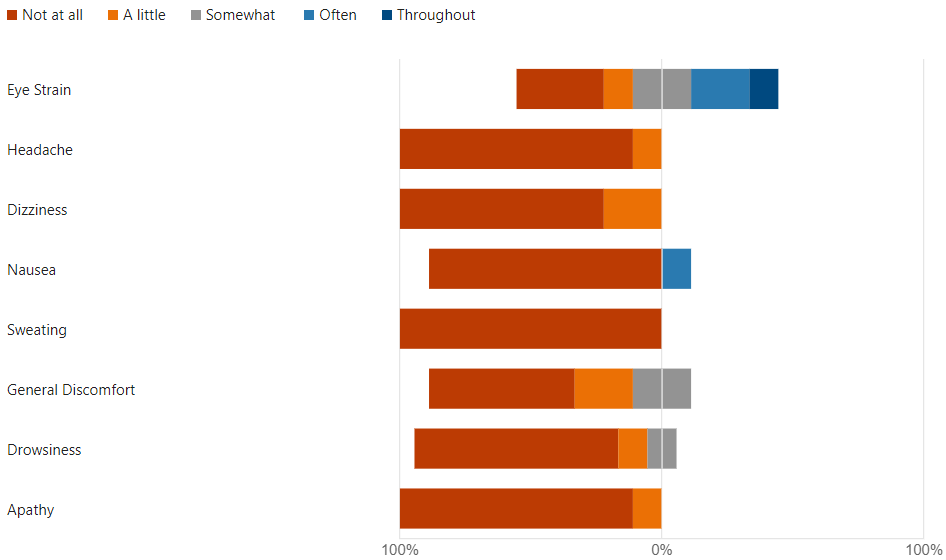
\includegraphics[width=\textwidth]{dissertation/images/Symptoms_Part_2.png}
        \caption{Responses after the users second eye was tested.}
        \label{fig:symptoms_part_2}
    \end{subfigure}
    \caption{Results from User Evaluation across both test conditions. Figure \ref{fig:symptoms_part_1} shows responses after the first eye was tested, with Figure \ref{fig:symptoms_part_2} showing responses after the second eye was tested.}
\end{figure}
\newpage
\subsection{Full Survey Results} \label{appendix:full_survey_results}
\begin{figure}[htbp]
    \centering
    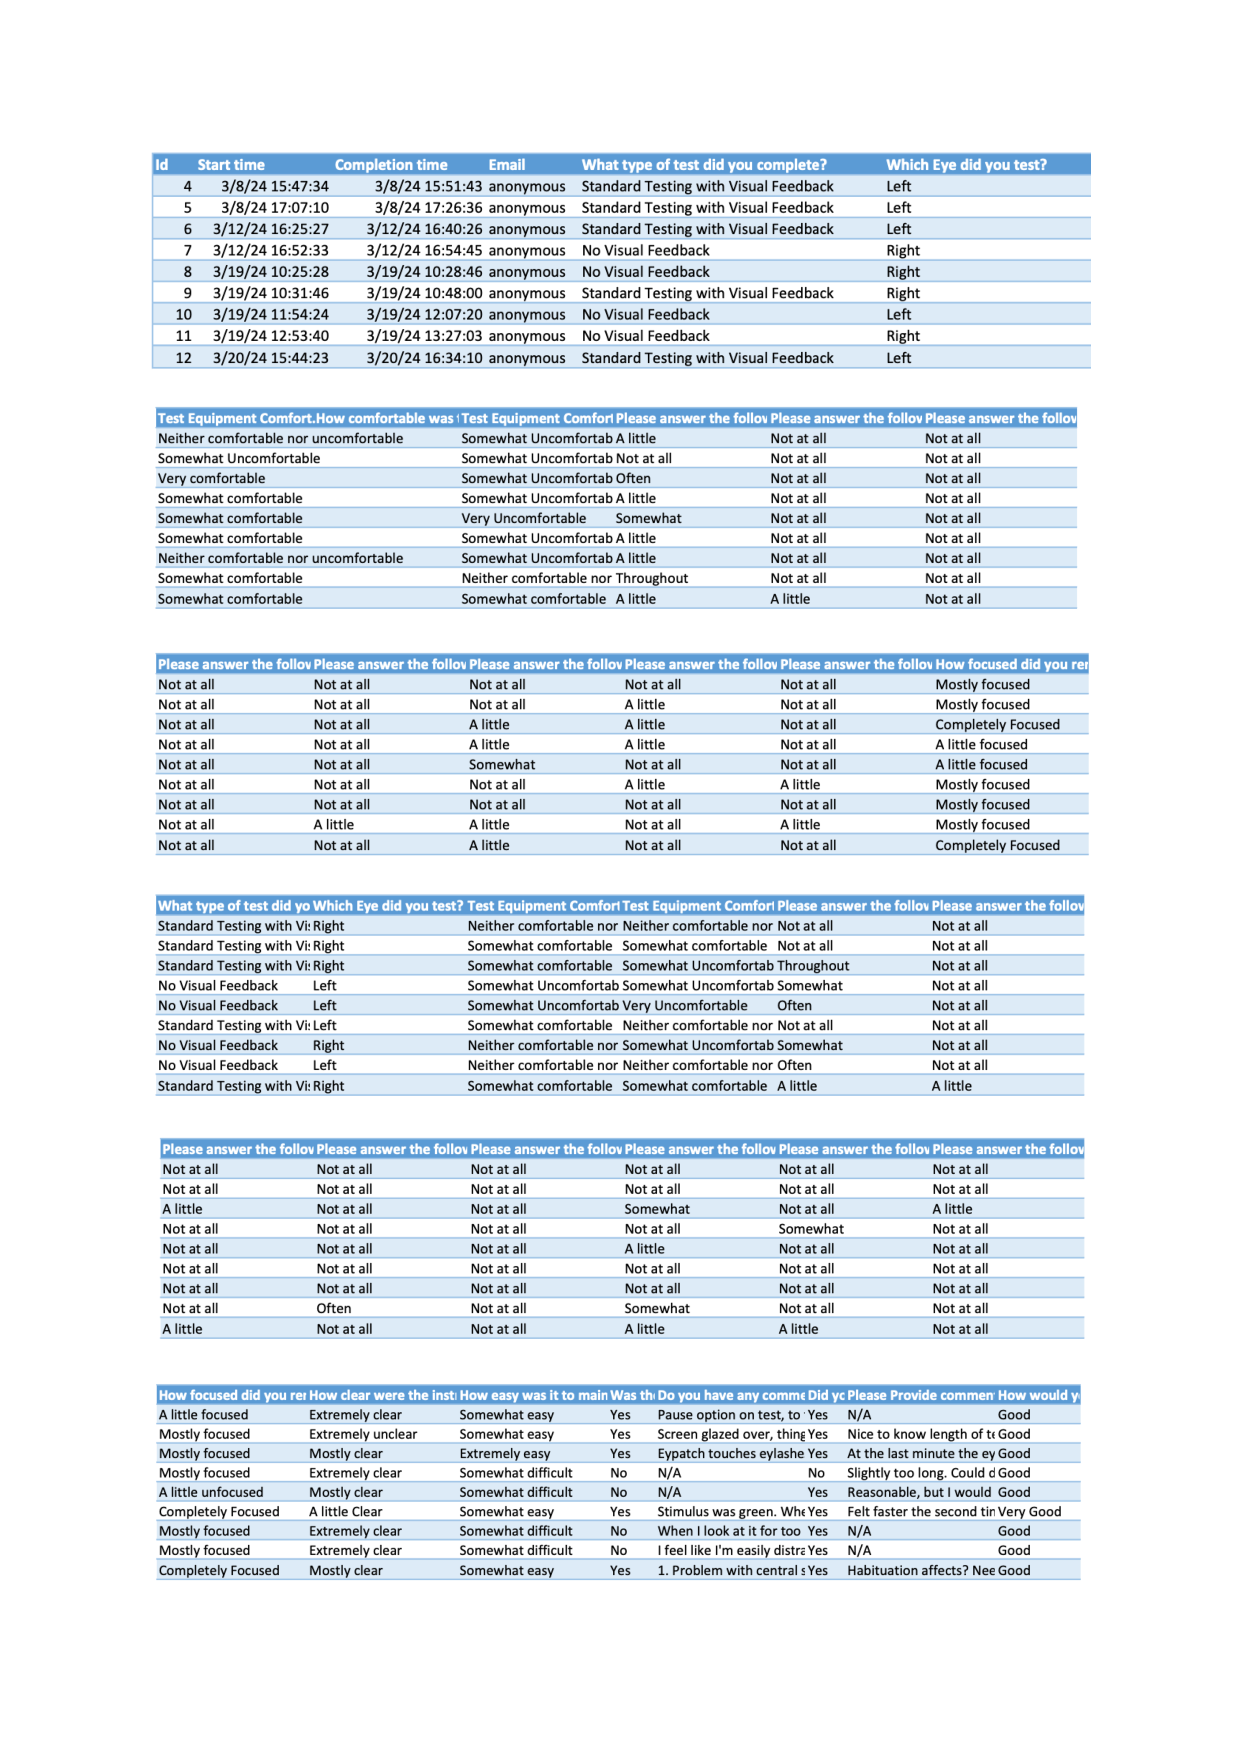
\includegraphics[page=1,width=1\linewidth]{dissertation/images/Full results.pdf}   
    \caption{Full survey results from user evaluation. Part 1/2.}
\end{figure}
\begin{figure}[htbp]
    \centering
    \includegraphics[page=2,width=1\linewidth]{dissertation/images/Full results.pdf}   
    \caption{Full survey results from user evaluation. Part 2/2.}
\end{figure}
\end{appendices}

%==================================================================================================================================
%   BIBLIOGRAPHY   

% The bibliography style is abbrvnat
% The bibliography always appears last, after the appendices.

\bibliographystyle{abbrvnat}

\bibliography{l4proj}

\end{document}
